%% Adaptative QITE -- status report of the work completed through Phase V.
%% Build (from this folder):
%%   latexmk -pdf -interaction=nonstopmode Adaptative_QITE_Status_Report.tex
%% Figures are read in place from the project's figure folders (see \graphicspath).
\documentclass[aps,pra,reprint,superscriptaddress,nofootinbib]{revtex4-2}

\usepackage[utf8]{inputenc}
\usepackage[T1]{fontenc}
\usepackage{amsmath,amssymb}
\usepackage{booktabs}
\usepackage{graphicx}
\usepackage{xcolor}
\usepackage[colorlinks=true,linkcolor=blue!50!black,citecolor=blue!50!black,urlcolor=blue!50!black]{hyperref}

\graphicspath{%
  {../Replications/practical-limitations-qdp/figures/}%
  {../Attack_Route_03/figures/}%
  {../Adam_QITE/figures/}%
  {../Replications/Beyond_Trot/figures/}%
  {../Route_03_and_Beyond_Trot/Proposal_1/figures/}%
  {../Route_03_and_Beyond_Trot/Proposal_2/figures/}%
}

\newcommand{\dt}{\Delta\tau}
\newcommand{\thetadot}{\dot\theta}
\newcommand{\cond}{\mathrm{cond}}
\newcommand{\Tr}{\mathrm{Tr}}
\newcommand{\rcond}{\texttt{rcond}}
\newcommand{\tol}{\mathrm{tol}}
\newcommand{\Efloor}{E_{\mathrm{floor}}}
\newcommand{\verdict}[1]{\textsl{#1}}

\begin{document}

\title{Adaptive time-stepping for variational quantum imaginary-time evolution:\\
 report on the work completed}

\begin{abstract}
Variational quantum imaginary-time evolution (QITE) integrates the linear system
$M\thetadot=Y$ given by McLachlan's principle. Both the step size $\dt$ and the conditioning of
the metric $M$ decide whether a run is accurate and how much it costs. This report collects,
phase by phase, what the project has done through Phase~V and what it found. All results are for H$_2$
in STO-3G on two qubits. The work falls into five phases. \emph{(I)} Replicated Saxena,
Shalabi and Kyaw's noise-scaling analysis. Theorem~1 and the noisy-flow scaling reproduce to
$10^{-10}$. The quoted condition numbers do not reproduce ($863.26$ against $66.72$), and the
9-parameter metric is exactly rank~6 of 9. It was found that Theorem~2 overstates the
hardware error by exactly a factor of two. \emph{(II)} An Adam-like step controller was built
and audited. Read at the circuit budget where the simpler ratchet controller finishes, it wins in every case
tested; at 732 circuits the two differ by only $3\times10^{-5}$. Two headline claims were withdrawn. One positive result was confirmed: a zero-cost
local-error estimator tracks step doubling with log-Pearson correlation $0.9902$, at the
predicted ratio of~2. \emph{(III)} A physics-indicator controller (Route~3) was implemented
and audited. At a matched budget of 732 circuits it lands $2.2\times$ closer to the variational floor than
fixed-step Euler. A debiasing ``surprise'' was traced to a wrong bias factor and retracted,
and so was a claimed noise floor. \emph{(IV)} Replication of Assi, Vogl, Kumari and LeBlanc's
variational product formulas. Their figures reproduce to ${\lesssim}1.2\%$, but four internal inconsistencies were found in the paper, and the unreported metric condition number reaches $10^{16}$ in a boundary
layer. \emph{(V)} Two pre-registered experiments followed. They show that the Route-3 stiffness
is a chart singularity of the parametrization, not a numerical error. They also show that
the end-point error does not track a requested tolerance, for reasons identified. Every
number quoted is pinned by a verification script that has no tolerance parameter, except a few single-run checks labelled as such (Sec.~\ref{sec:scope}).
\end{abstract}

\maketitle

%% ===========================================================================
\section{Introduction}
\label{sec:intro}

Imaginary-time evolution $|\psi(\tau)\rangle\propto e^{-H\tau}|\psi_0\rangle$ drives any state
with nonzero ground-state overlap to the ground state of $H$~\cite{Motta2020,Arulandu2026}. The variational form of QITE
restricts the state to a parametrized circuit $|\psi(\theta)\rangle$. McLachlan's principle
then gives an ordinary differential equation for the parameters~\cite{McArdle2019,QDP2024,Angles2025},
\begin{equation}
  M(\theta)\,\thetadot = Y(\theta),
  \label{eq:mclachlan}
\end{equation}
with $M$ the (real part of the) quantum geometric tensor and $Y$ an energy-gradient vector.
On hardware each evaluation of $\thetadot=f(\theta)=M^{+}Y$ costs $O(N^2)$ circuits for $N$
parameters. The step size therefore sets the circuit bill directly. The quality of the
linear solve depends on $\cond(M)$ and on the cutoff used in the pseudo-inverse.

The project starts from \emph{Adaptive Time-Stepping for
Variational QITE: An RKF-Type Controller with a Hardware-Noise Floor}~\cite{Memo}, hereafter the memo.
The memo treats Eq.~\eqref{eq:mclachlan} as an ODE integrated by a Runge--Kutta--Fehlberg-type
controller, and it adds a noise floor derived from the Saxena--Shalabi--Kyaw (QDP) bounds~\cite{QDP2024}.
It proposes five attack routes. This report documents what has been built, measured,
audited and corrected on top of it. It is organized by phase (Table~\ref{tab:chronology}).

\paragraph*{Main established results.}
\begin{enumerate}
\setlength\itemsep{0pt}
\item The QDP noise-scaling results (Theorem~1 and the noisy-flow scaling) reproduce to about
  $10^{-10}$. On hardware, where the state inside $\{H,\rho\}$ is also noisy, the parameter-velocity
  error is \emph{exactly half} of what Theorem~2 states (Sec.~\ref{sec:phase1}).
\item The QDP ansätze are far worse conditioned than reported. The 5-parameter metric has
  $\cond_F=863.26$, not $66.72$. The 9-parameter metric is exactly rank~6 of~9, which is
  structural because a two-qubit pure state has $2d-2=6$ real degrees of freedom.
\item A zero-cost local-truncation-error estimator is already available in any energy-gated
  controller. It agrees with step doubling at the predicted ratio of~2 (Sec.~\ref{sec:phase2}).
\item Adding momentum (Adam-style EMAs) to the step-size law does not beat a simple ratchet at
  matched circuit budget (Sec.~\ref{sec:phase2}).
\item At a matched budget of 732 circuits, a cap based on $\cond(M)$ plus a variational energy gate lands $2.2\times$
  closer to the variational floor than fixed-step Euler (Sec.~\ref{sec:phase3}).
\item The large-$\cond(M)$ events in the 9-parameter runs are a chart singularity. The
  parameter speed diverges while the state speed stays bounded. They are not gauge leakage and
  not finite-difference noise (Sec.~\ref{sec:phase5}).
\item With a proportional--integral (PI) law and an explicit tolerance, the controller does
  regulate its local-error estimate. The error at the final time still does not scale with
  the tolerance, because the flow is contractive and the first step is fixed
  (Sec.~\ref{sec:phase5}).
\end{enumerate}

\begin{table*}[t]
\caption{The project by phase. ``Pinned'' counts the numerical values checked by the phase's verification script
(Appendix~\ref{app:repro}).}
\label{tab:chronology}
\begin{ruledtabular}
\begin{tabular}{lp{5.2cm}p{7.4cm}}
Phase & Work & Outcome \\
\midrule
I   & Replication of Saxena--Shalabi--Kyaw~\cite{QDP2024} (T1--T5)
    & T1, T4 reproduced; T2, T5 partially; T3 not reproduced. Factor-of-two correction to Theorem~2. \\
II  & Adam-like step controller (E1--E3); audit G1--G7
    & Ratchet wins at matched completion budget; E2 withdrawn, E3 re-attributed; zero-cost error estimator
      validated; 147 values pinned, 0 drift. \\
III & Route-3 controller (Targets A--D); audit F1--F12, modules M1--M6
    & $2.2\times$ closer to floor at 732 circuits; debias factor corrected; tight \rcond{} beats loose
      by $2.4\times$; noise-floor claim retracted. \\
IV  & Replication of Assi--Vogl--Kumari--LeBlanc~\cite{BeyondTrot2026} (T1--T8)
    & Figures reproduce; four internal inconsistencies found; $\cond(g)$ boundary layer (T6) pinned. \\
V   & P1 (singularity classification); P2 (tolerance proportionality)
    & Chart singularity, no gauge leakage (51 pinned); no tolerance fit possible, post-hoc
      first-step ablation (93 pinned). \\
\end{tabular}
\end{ruledtabular}
\end{table*}

%% ===========================================================================
\section{Framework and methods}
\label{sec:methods}

\subsection{Variational QITE and the linear solve}

For a density matrix $\rho(\theta)$ the metric and gradient are~\cite{QDP2024}
\begin{align}
  M_{kq} &= \Tr\!\left[\partial_k\rho\,\partial_q\rho\right], \label{eq:M}\\
  Y_k &= -\Tr\!\left[\partial_k\rho\left(\{H,\rho\}-2\langle H\rangle\rho\right)\right]. \label{eq:Y}
\end{align}
For a pure state $\partial_k\rho=|\partial_k\psi\rangle\langle\psi|+|\psi\rangle\langle\partial_k\psi|$,
and normalization makes $\langle\partial_k\psi|\psi\rangle$ purely imaginary. Equation~\eqref{eq:Y}
then collapses to
\begin{equation}
  Y_k = -\partial_k E,\qquad E(\theta)=\langle\psi(\theta)|H|\psi(\theta)\rangle,
  \label{eq:Ygrad}
\end{equation}
which was verified numerically to $\|Y+\nabla E\|/\|Y\|=2.3\times10^{-10}$. For a product of
Pauli rotations with generators $\tilde G_k$ (dressed by the gates to their left),
\begin{equation}
\begin{gathered}
  M_{jk}=2\left(\mathrm{Re}\langle\tilde G_j\tilde G_k\rangle-\langle\tilde G_j\rangle\langle\tilde G_k\rangle\right),\\
  Y_k=-i\langle[\tilde G_k,H]\rangle,
\end{gathered}
  \label{eq:stateform}
\end{equation}
which was checked against the finite-difference $M$ and $Y$ to $2.594\times10^{-10}$ and $3.955\times10^{-10}$
(Sec.~\ref{sec:phase5}).

Equation~\eqref{eq:mclachlan} is integrated with explicit Euler,
$\theta_{n+1}=\theta_n+\dt_n\,M^{+}Y$. The pseudo-inverse cutoff \rcond{} (relative to the
largest singular value) is always an explicit, logged parameter, and the reported $\cond(M)$
is always stated as either the regularized Frobenius value $\cond_F$ or the unregularized
spectral value. Section~\ref{sec:phase5} shows that this distinction is significant.

\subsection{Noise model and the QDP bounds}

Following Ref.~\cite{QDP2024}, every gate is followed by the global depolarizing channel
$\mathcal E(\rho)=(1-p)\rho+p\,\mathbb{I}/d$, with $d=4$. After $N$ gates, and writing
$q\equiv(1-p)^N$,
\begin{equation}
  \rho^{\mathrm{err}} = q\,\rho + (1-q)\,\mathbb{I}/d .
  \label{eq:depol}
\end{equation}
Theorem~2 of Ref.~\cite{QDP2024} states that the relative velocity error is
$\epsilon/\|\thetadot\|=(1-q)/q$, independent of the Hamiltonian. Theorem~1 bounds the same
error in terms of $\|M\|$, $\|M^{-1}\|$ and $\|Y\|$. The memo inverts the Theorem-2 bias as
$\tilde f=q^{-1}f$ (memo Eq.~7) and combines truncation and residual error into
\begin{equation}
  e_n^2\approx C_{\mathrm{tr}}^2\dt^{2(p+1)}+\dt^2\kappa_b^2\varepsilon_{\mathrm{res}}^2\|\thetadot\|^2,
  \label{eq:memo8}
\end{equation}
where $p$ is the order of the integrator (memo Eq.~8). Below the resulting $\dt_{\mathrm{floor}}$,
shrinking the step does not help (memo Eq.~9). The memo's Route~3 replaces the RKF error estimate
with physics indicators: the McLachlan residual, energy monotonicity
$dE/d\tau=-2\,\mathrm{Var}_\rho(H)$ (memo Eq.~13), and $\cond(M)$ as a stiffness proxy. Its
Route~4 proposes the PI law
\begin{equation}
  \dt_{n+1}=\dt_n\left(\frac{\tol}{e_n}\right)^{k_I}\left(\frac{e_{n-1}}{e_n}\right)^{k_P},
  \label{eq:PI}
\end{equation}
with $k_I\approx0.3/(p+1)$ and $k_P\approx0.4/(p+1)$ (memo Eq.~17).

\subsection{Baseline step law (Route 3)}
\label{sec:baseline}

All controllers in this report are compared with a common baseline, which is called Route~3 throughout this document.
It is the implementation of the memo's third route. The memo gives no numbers and no rule for
combining the indicators, so both the rule and every constant in Table~\ref{tab:constants} are
heuristic choices. Each iteration does the following.
\begin{enumerate}
\setlength\itemsep{0pt}
\item \textbf{Stiffness cap (proactive).} Measure $M$ and $Y$ and solve. Then set
  $\dt\leftarrow\max\!\big(\dt_{\min},\min(\dt,\,c_{\mathrm{cap}}/\cond(M),\,\dt_{\max})\big)$.
  A singular $M$ ($\cond=\infty$) sends $\dt$ to the floor, not to zero.
\item \textbf{Energy gate (reactive).} Take the trial step and compare the energy change
  $\Delta E_a$ with the variational first-order prediction $\Delta E_p=-(Y\cdot\thetadot)\dt$.
  If $E$ rises by more than a monotonicity tolerance, or if $|\Delta E_a-\Delta E_p|$ exceeds
  $\max(\text{ABS},\text{REL}\,|\Delta E_p|)$, shrink $\dt$ by $1/2$ and retry, up to 20 times.
  If the retries run out, the last trial is committed.
\item \textbf{Ratchet.} After an accepted step, multiply $\dt$ by 1.25 unless the relative
  McLachlan residual exceeds 5\%, in which case growth is frozen. The residual never triggers
  a retry.
\end{enumerate}

\begin{table}[b]
\caption{Constants of the baseline step law. None comes from the memo; all were chosen for this work.}
\label{tab:constants}
\begin{ruledtabular}
\begin{tabular}{lll}
Constant & Value & Role \\
\midrule
$\dt_0$ & 0.05 & initial step \\
$\dt_{\min}$, $\dt_{\max}$ & $10^{-4}$, 0.5 & clip range \\
GROW, SHRINK & 1.25, 0.5 & ratchet, retry \\
$c_{\mathrm{cap}}$ & 2000 & stiffness cap $c_{\mathrm{cap}}/\cond(M)$ \\
\rcond{} (default) & $10^{-6}$ & pseudo-inverse cutoff \\
monotonicity tol. & $10^{-9}$ & energy may not rise \\
ABS, REL & $10^{-3}$, 0.5 & energy-gate band \\
residual tol. & 0.05 & freezes growth \\
max.\ retries & 20 & per step \\
\end{tabular}
\end{ruledtabular}
\end{table}

The cap coefficient was first set to 50. At that value the cap dominated the whole run, so it
was raised to 2000. The gate originally tested against the exact-ITE identity
$-2\,\mathrm{Var}(H)\dt$. The audit (F5) replaced this with the variational prediction,
because the ansatz deficit does not vanish at convergence. The baseline described here is the post-audit version.

\subsection{Benchmark}

All runs use H$_2$ in STO-3G under the Bravyi--Kitaev mapping, reduced to two qubits, with the
5-parameter and 9-parameter ansätze of Ref.~\cite{QDP2024}. Derivatives $\partial_k\rho$ are
central finite differences with $h=10^{-6}$. They are validated against the closed-form
diagonal $M_{kk}=\tfrac12(1-\Tr[P_k\rho P_k\rho])$ (Eq.~B9 of Ref.~\cite{QDP2024}), with a
worst deviation of $8.9\times10^{-11}$. Simulations use PennyLane~0.45.1 with fixed seeds, and
each target has its own seed. $\Efloor=-1.124600$ is the variational minimum of the 5-parameter
ansatz, obtained by direct minimization. It lies $2.100\times10^{-2}$ above the exact ground-state energy. 
Convergence against $\Efloor$ is reported because no controller can get past it.

\subsection{Evidence protocol}
\label{sec:protocol}

Every figure, table entry or claimed number has its own function in a script. Verdicts use
three words: \verdict{reproduced}, \verdict{partially reproduced} and
\verdict{not reproduced}. Every quoted value is pinned in a verification script, and a
\texttt{--check} mode re-runs the computation and compares against the pinned values with no
adjustable tolerance. From Phase~V on, predictions were registered in writing before the run,
and their outcomes are scored as held or failed. Controllers are compared in a common currency
of \emph{circuits}. One evaluation of $f$ with $N$ parameters costs $2N+1$ circuits, and each energy-gate trial, including the first, costs one more. Comparisons ``at matched budget'' read every run at the same
circuit count.

%% ===========================================================================
\section{Phase I: replication of the QDP noise analysis}
\label{sec:phase1}

\paragraph*{Question.} Does the noise-scaling analysis on which the memo builds its floor
reproduce, and does it apply as stated to hardware?

\paragraph*{Summary.} Table~\ref{tab:qdp} lists the targets. The closed-form results reproduce,
while the numbers that depend on unstated details do not.

\begin{table}[t]
\caption{Phase I verdicts for Ref.~\cite{QDP2024}.}
\label{tab:qdp}
\begin{ruledtabular}
\begin{tabular}{p{3.9cm}l}
Target & Verdict \\
\midrule
T1: Theorem~1 bound, Eq.~(17) & \verdict{reproduced} \\
T2: $p_{\max}$ at $\delta=0.04$, $N=5$--$14$ & \verdict{partially reproduced} \\
T3: $\cond(M)$, 5- and 9-param.\ ansätze & \verdict{not reproduced} \\
T4: noisy flow vs Eq.~(19) & \verdict{reproduced} ($\sim10^{-10}$) \\
T5: Fig.~3(b) Theorem-1 curves & \verdict{partially reproduced} \\
\end{tabular}
\end{ruledtabular}
\end{table}

\paragraph*{T2: maximal noise rate.} All five values of $p_{\max}$ come out between 1.4\% and
3.5\% \emph{above} the paper's (Table~\ref{tab:qdp_t2}). The offset is one-sided. Back-solving
$\|M\|$ from each paper value gives $1.1018$, $1.0456$, $1.0947$, $1.0631$ and $1.0075$, which
are mutually inconsistent. A common rescaling of $\|M\|$ therefore cannot explain the gap. The
pattern is consistent with the paper quoting the last point of a discrete $p$ grid that still
satisfies the bound.

\begin{table}[t]
\caption{T2: $p_{\max}$ at $\delta=0.04$.}
\label{tab:qdp_t2}
\begin{ruledtabular}
\begin{tabular}{rlll}
$N$ & paper & this work & deviation \\
\midrule
5  & 0.032 & 0.03311 & $+3.48\%$ \\
6  & 0.036 & 0.03653 & $+1.48\%$ \\
10 & 0.052 & 0.05349 & $+2.86\%$ \\
12 & 0.068 & 0.06964 & $+2.41\%$ \\
14 & 0.129 & 0.13083 & $+1.42\%$ \\
\end{tabular}
\end{ruledtabular}
\end{table}

\paragraph*{T3: conditioning of the ansätze.} For the 5-parameter ansatz the replication gives
$\cond_F=863.2577$ against the paper's $66.7239$ ($+1194\%$). The corresponding values are
$\|M\|_F=0.8793$ (paper $0.9977$) and spectral condition number $624.9$. Because a condition number is scale-free, no normalization convention can close this gap. A
60-row scan over the choices the paper leaves open (initial state, controlled or Ising
two-qubit gate, wire order, and three metric conventions) gives values clustered at
$863.26$, $879.59$ and $911.08$. None of them lands within 5\% of the paper. The 9-parameter
ansatz is worse. Its singular values are
\begin{multline*}
[1.267,\,0.706,\,0.633,\,0.383,\,0.181,\,0.0432,\\
8.8{\times}10^{-17},\,2.9{\times}10^{-17},\,3.2{\times}10^{-18}],
\end{multline*}
so $M$ has rank~6 and $\cond(M)=\infty$, where the paper reports $20.22$. The rank deficiency is
structural. The pure states of two qubits form a manifold of real dimension $2d-2=6$, so any
9-parameter ansatz carries at least three gauge directions. A finite value such as the
paper's is therefore a property of the pseudo-inverse cutoff, not of the ansatz. The
regularized value is $39.41$ for every \rcond{} from $10^{-15}$ to $10^{-2}$, then $10.69$ at
$0.1$ and $5.66$ at $0.3$. None matches $20.22$. The same ansatz gives $\|M\|_F=1.6387$
(paper $1.689$) and $\|Y\|=0.1927$ (paper $0.121$).

\paragraph*{T4: the noisy flow.} Simulating the circuit with a depolarizing channel after every
gate reproduces Eq.~(19) of Ref.~\cite{QDP2024} to about $10^{-10}$. The residuals are
$M^{\mathrm{err}}\le4\times10^{-10}$ and $Y^{\mathrm{err}}\le10^{-9}$, with a largest
$\thetadot$ deviation of $2.8\times10^{-7}$ (Fig.~\ref{fig:t4}, circles).

\paragraph*{T5: Theorem-1 curves.} Fig.~3(b) of Ref.~\cite{QDP2024} can be read in at least
three ways (Table~\ref{tab:qdp_t5}). The reading that drops the $\|Y\|$ term is closest to the
figure. None matches it at every $N$. The denominator of Eq.~(A42) is also positive only for
$p\le4.28\times10^{-4}$ ($N=5$) down to $p\le6.68\times10^{-5}$ ($N=14$), which is below most
of the plotted range.

\begin{table}[t]
\caption{T5: Fig.~3(b) read-offs against three readings of Eq.~(17).}
\label{tab:qdp_t5}
\begin{ruledtabular}
\begin{tabular}{lrrrrr}
 & $N{=}5$ & 6 & 10 & 12 & 14 \\
\midrule
Fig.~3(b) read-off & 75 & 105 & 300 & 430 & 590 \\
Eq.~(17) as printed & 103.4 & 146.6 & 396.6 & 575.3 & 824.3 \\
Eq.~(17) per (A37) & 119.0 & 168.8 & 457.0 & 665.9 & 969.5 \\
$\|Y\|$ term dropped & 77.2 & 109.7 & 295.7 & 423.9 & 581.7 \\
\end{tabular}
\end{ruledtabular}
\end{table}

\begin{figure}[t]
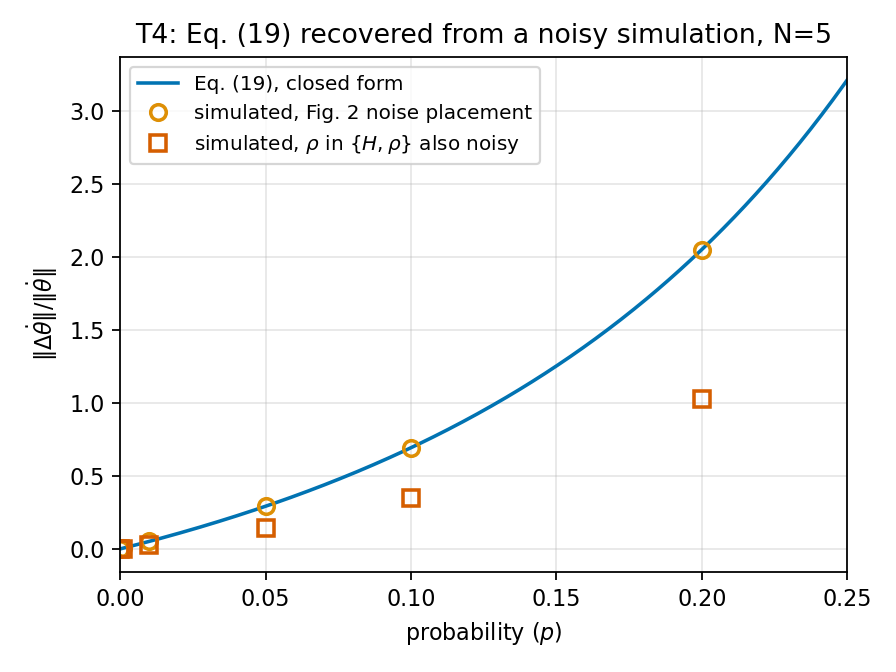
\includegraphics[width=\columnwidth]{t4_scaling}
\caption{T4 and the factor of two ($N=5$). The line is the closed form of Eq.~(19) in
Ref.~\cite{QDP2024}. Circles are the simulated relative velocity error with noise placed as
in the paper's Fig.~2, where only $\partial_k\rho$ is noisy. Squares have the state inside
$\{H,\rho\}$ noisy as well, as it is on hardware. The squares sit at exactly half the
closed form.}
\label{fig:t4}
\end{figure}

\paragraph*{New result: Theorem 2 is a factor of two pessimistic on hardware.} The derivation
in Appendix~B of Ref.~\cite{QDP2024} applies noise to the derivative $\partial_k\rho$ but
keeps the state in $\{H,\rho\}$ ideal. On hardware both come from the same noisy device.
Using Eq.~\eqref{eq:depol} for both, with $\Tr\,\partial_k\rho=0$ and
$\Tr[\partial_k\rho\,\rho]=0$ (Appendix~\ref{app:factor2}), gives
\begin{align}
  M^{\mathrm{err}} &= q^2 M, \qquad Y^{\mathrm{err}} = \Big[q^2+\tfrac{2}{d}q(1-q)\Big]Y,\\
  \thetadot^{\mathrm{err}} &= \thetadot\left[1+\frac{1-q}{2q}\right]\quad(d=4),
  \label{eq:factor2}
\end{align}
so the relative error is $(1-q)/(2q)$, exactly half of Theorem~2's $(1-q)/q$. Numerically,
the ratio of the two errors equals $0.5$ to within $3.8\times10^{-5}$ across
$p\in[10^{-4},0.2]$ (Fig.~\ref{fig:t4}, squares). The consequence for the memo is concrete:
its debiasing factor $q^{-1}$ (memo Eq.~7) over-corrects on hardware. The correct factor is
$\big[q^2+q(1-q)/2\big]/q^2$. Phase~III first missed this and then corrected it.

%% ===========================================================================
\section{Phase II: Adam-like step controller and its audit}
\label{sec:phase2}

\paragraph*{Question.} Can the step-size law of the baseline (Sec.~\ref{sec:baseline}) be
improved by adding the memory of the Adam optimizer, that is, by smoothing the error signal
before acting on it?

\subsection{Design}

The controller keeps Route~3's cap, gate and thresholds and replaces only the ratchet. It uses
the energy-gate discrepancy, normalized by the gate band, as an error signal:
\begin{equation}
  \hat e_n=\frac{|\Delta E_a-\Delta E_p|}{\max(\text{ABS},\,\text{REL}\,|\Delta E_p|)} .
  \label{eq:ehat}
\end{equation}
Bias-corrected exponential moving averages $\hat m_e$ and $\hat v_e$ of $\hat e$ and $\hat e^2$
($\beta_1=0.9$, $\beta_2=0.999$, $\varepsilon=10^{-8}$) define a confidence ratio
$s_e=\hat m_e/(\sqrt{\hat v_e}+\varepsilon)$. The growth factor is
\begin{equation}
  \text{growth}=\max(\hat m_e,\varepsilon)^{-s_e k_I},\qquad k_I=0.15,
  \label{eq:adamlaw}
\end{equation}
clipped to $[0.5,1.25]$. A parallel EMA of the residual only sets a ceiling on growth. The
Adam machinery acts on the scalar $\dt$ alone and never rescales individual parameters. A
per-parameter rescaling would change the ODE being integrated, which would make it a
different method, not a step controller for the same one.

\paragraph*{Consistency check.} With $\beta_1=\beta_2=0$ and $k_I=10$, the controller
reproduces Route~3 exactly (172 steps, final $E=-1.122993$). A memoryless variant gives 172
steps and $-1.122928$.

\subsection{Experiments as first reported}

Three experiments were run. E1 compares convergence on the noiseless 5-parameter ansatz
(Fig.~\ref{fig:e1}). E2 compares behaviour under depolarizing noise. E3 compares behaviour on
the rank-deficient 9-parameter ansatz (Fig.~\ref{fig:e3}). The first report credited Adam with
a small E1 advantage at 732 circuits ($-1.121027$ against $-1.120992$), with robustness to
noise in E2, and with a better cap-off result in E3.

\begin{figure*}[t]
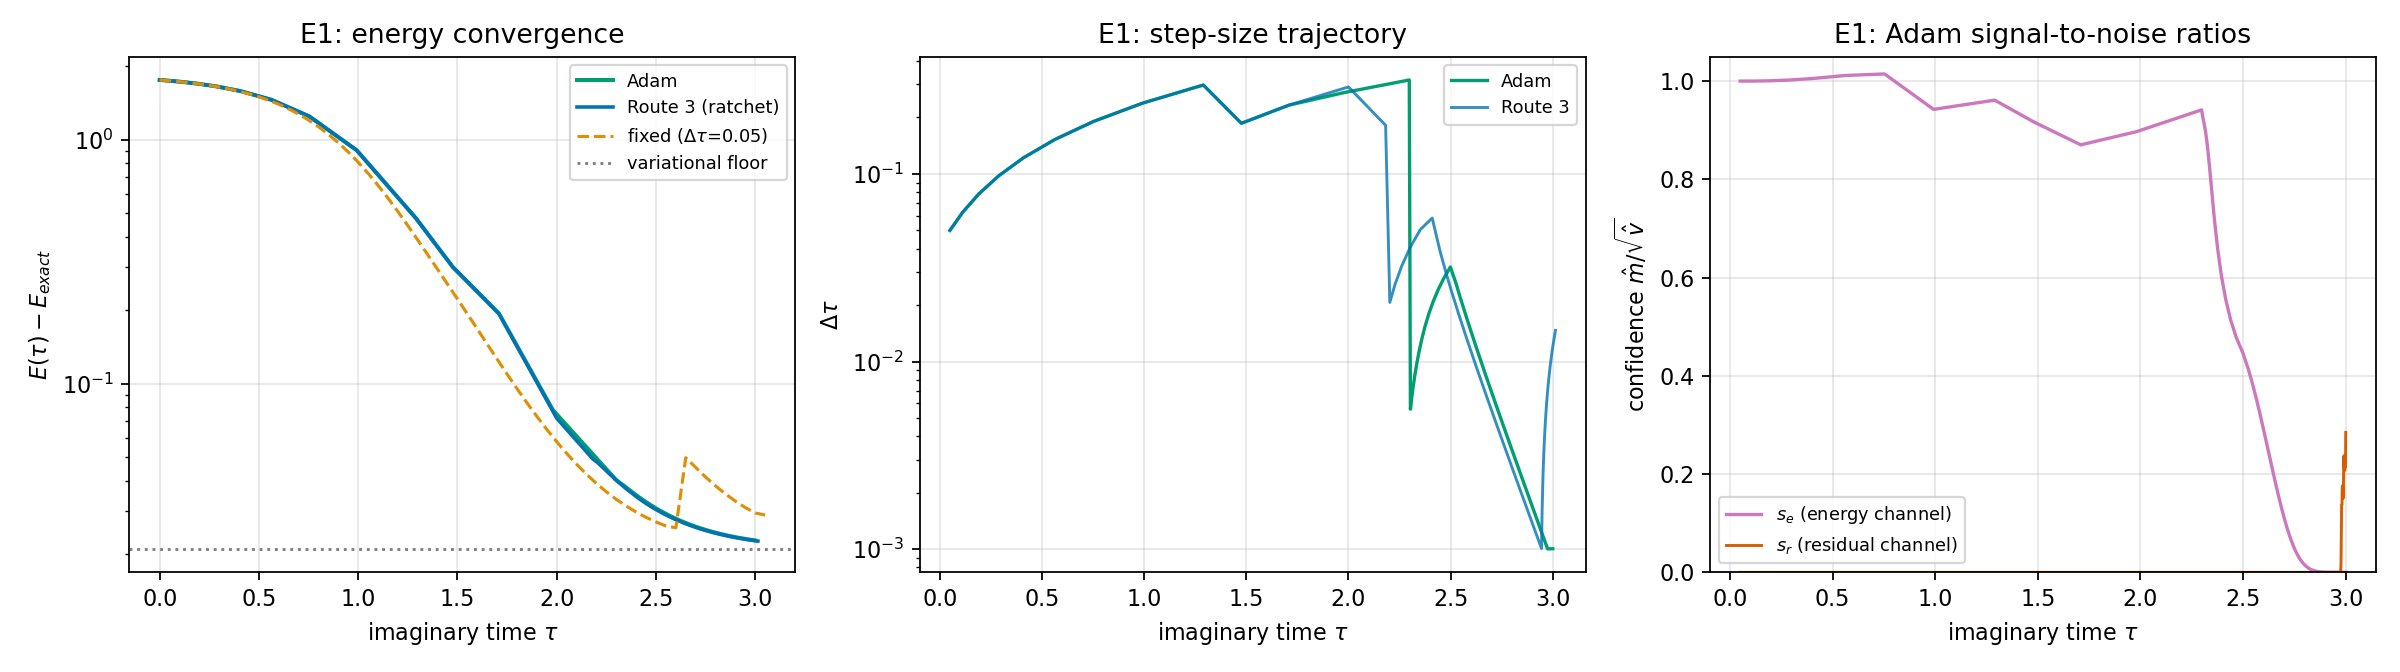
\includegraphics[width=\textwidth]{target_e1_controllers}
\caption{E1, noiseless 5-parameter ansatz. Left: energy above the exact ground state for the
Adam controller, Route~3 and fixed-step Euler ($\dt=0.05$). The dotted line is the variational
floor. Centre: step-size trajectories. Right: the Adam confidence ratios. The energy channel
$s_e$ decays to zero after $\tau\approx2.3$, which is the ``frozen'' regime discussed in the
text.}
\label{fig:e1}
\end{figure*}

\subsection{Audit (G1--G7) and what it changed}

A full audit re-ran every claim against live code. It produced seven findings,
G1--G7. The consequential ones follow.

\paragraph*{G2: the $\beta_2$ horizon decides every verdict.} With $\beta_2=0.999$ the second
moment has an effective memory of about 1000 steps, longer than any run. $\sqrt{\hat v_e}$ is
then set by a much longer memory than $\hat m_e$, and $s_e$ collapses toward zero. The ``frozen'' fraction in
Table~\ref{tab:g2} counts the steps where this happens. The table repeats E1 on two seeds at
matched circuit budget, for the stock setting and for three settings with equal horizons.
\emph{Read at Route~3's completion budget (2069 and 2816 circuits), Route~3 wins in every case.} The stock Adam arm on the second seed does
not reach $\tau_{\max}$ within 500 steps. With equal $\beta$'s, Adam ends slightly below
Route~3 in final energy, but only after spending more circuits.

\begin{table*}[t]
\caption{G2: E1 at matched circuit budget on two seeds. ``$E-\Efloor$'' is at the end of each
run; ``at budget'' reads each run at the circuit count Route~3 used. $\langle s_e\rangle$ is the
mean confidence ratio; ``frozen'' is the fraction of steps with $s_e$ effectively zero.}
\label{tab:g2}
\begin{ruledtabular}
\begin{tabular}{llrrlllr}
Seed (budget) & Arm & Steps & Circuits & $E-\Efloor$ & at budget & $\langle s_e\rangle$ & frozen \\
\midrule
A (2069) & Route 3 & 172 & 2069 & $+1.607\times10^{-3}$ & $+1.607\times10^{-3}$ & -- & -- \\
 & Adam $0.9/0.999$ (stock) & 190 & 2285 & $+1.748\times10^{-3}$ & $+1.860\times10^{-3}$ & 0.140 & 49\% \\
 & Adam $0.9/0.9$ & 179 & 2151 & $+1.190\times10^{-3}$ & $+1.800\times10^{-3}$ & 0.200 & 0\% \\
 & Adam $0.99/0.99$ & 184 & 2212 & $+1.437\times10^{-3}$ & $+1.841\times10^{-3}$ & 0.355 & 0\% \\
 & Adam $0.999/0.999$ & 181 & 2176 & $+1.447\times10^{-3}$ & $+1.803\times10^{-3}$ & 0.407 & 0\% \\
\midrule
D (2816) & Route 3 & 234 & 2816 & $+8.555\times10^{-4}$ & $+8.555\times10^{-4}$ & -- & -- \\
 & Adam $0.9/0.999$ (stock) & 500 & 6006 & $+1.598\times10^{-3}$ & $+4.165\times10^{-3}$ & 0.089 & 72\% \\
 & Adam $0.9/0.9$ & 244 & 2934 & $+8.641\times10^{-4}$ & $+3.495\times10^{-3}$ & 0.394 & 0\% \\
 & Adam $0.99/0.99$ & 259 & 3114 & $+8.637\times10^{-4}$ & $+3.942\times10^{-3}$ & 0.439 & 0\% \\
 & Adam $0.999/0.999$ & 254 & 3054 & $+8.430\times10^{-4}$ & $+3.893\times10^{-3}$ & 0.517 & 0\% \\
\end{tabular}
\end{ruledtabular}
\end{table*}

The horizon sweep on seed D (Table~\ref{tab:horizon}) makes the mechanism visible. Every
equal-horizon arm reaches $\tau_{\max}$ in about Route~3's number of steps. Reversing the
horizons ($\beta_1=0.999$, $\beta_2=0.9$) drives the mean $s_e$ to $258$. This also shows that
the bound $s_e\le1$ stated in the first report is false. Even in the stock E1 run $s_e$ spans
$[5.097\times10^{-5},\,1.015]$.

\begin{table}[t]
\caption{Horizon sweep, seed D. All arms except the stock one exit at $\tau_{\max}$; the stock arm exits at the 500-step limit.}
\label{tab:horizon}
\begin{ruledtabular}
\begin{tabular}{lrll}
Configuration & Steps & Final $E$ & $\langle s_e\rangle$ \\
\midrule
Route 3 & 234 & $-1.123745$ & -- \\
stock $0.9/0.999$ & 500 & $-1.123002$ & 0.0893 \\
$0.999/0.999$ & 254 & $-1.123757$ & 0.5170 \\
$0.99/0.99$ & 259 & $-1.123736$ & 0.4387 \\
$0.9/0.9$ & 244 & $-1.123736$ & 0.3938 \\
reversed $0.999/0.9$ & 242 & $-1.123740$ & 258.1220 \\
\end{tabular}
\end{ruledtabular}
\end{table}

\paragraph*{G4: the law cannot shrink the step.} In E1, $\hat e>1$ on 0 of 190 steps (maximum
$0.945$), and growth $<1$ on 0 of 190. This is not a tuning problem but an identity. The error
in Eq.~\eqref{eq:ehat} is normalized by the gate's own reject band, so $\hat e>1$ \emph{is} the
reject condition. The retry loop shrinks $\dt$ until the trial is in band, and the controller
is updated only after the loop exits. It therefore only ever observes $\hat e\le1$, so
$\hat m_e<1$ and growth $\ge1$ by construction (Appendix~\ref{app:shrink}). Moving the band over
three orders of magnitude, with gate and normalization moved together, left growth $<1$ at
$0/N$ at every setting. Any tolerance that serves at once as rejection threshold and control
setpoint is one-sided in this way. The E1 statistics show the scale mismatch as well: the
mean and median of $\hat e$ are $2.751\times10^{-2}$ and $2.902\times10^{-5}$, far below the
setpoint~1.

\paragraph*{G3: E2 cannot resolve noise.} Under the global depolarizing model the noisy flow is
a deterministic rescaling of the clean flow (Eq.~\eqref{eq:factor2}). There is no stochastic
component for an EMA to average out. The RMS ratios between Adam and Route~3 were
$1.0243$, $1.0246$, $1.0245$ and $1.0088$, independent of $p$ to $\pm0.016$. The E2 verdict,
and a reported ``stall'' that came from a metric artifact, are \emph{withdrawn}.

\paragraph*{G6: E3 is the cap, not Adam.} Table~\ref{tab:e3} gives the E3 runs. With the cap on,
Route~3 and Adam are identical to every printed digit, because the cap binds on the relevant
steps and neither growth law acts. The only difference appears with the cap \emph{off}. This is
a single run ($n=1$), the report had duplicate rows, and no cost-matched column was given. The
E3 advantage is therefore re-attributed to the cap and not claimed for Adam.

\begin{table}[t]
\caption{E3: 9-parameter ansatz. Error is $E-E_{\mathrm{exact}}$ at the end of the run.}
\label{tab:e3}
\begin{ruledtabular}
\begin{tabular}{llllr}
\rcond & Arm & Final $E$ & Error & Steps \\
\midrule
$10^{-8}$ & Route 3, cap on  & $-1.144712$ & $8.868\times10^{-4}$ & 108 \\
          & Route 3, cap off & $-1.144201$ & $1.398\times10^{-3}$ & 22 \\
          & Adam, cap on     & $-1.144712$ & $8.868\times10^{-4}$ & 108 \\
          & Adam, cap off    & $-1.145034$ & $5.653\times10^{-4}$ & 28 \\
\midrule
$10^{-2}$ & Route 3 & $-1.143456$ & $2.143\times10^{-3}$ & 17 \\
          & Adam    & $-1.142285$ & $3.314\times10^{-3}$ & 14 \\
\end{tabular}
\end{ruledtabular}
\end{table}

\begin{figure*}[t]
\centering
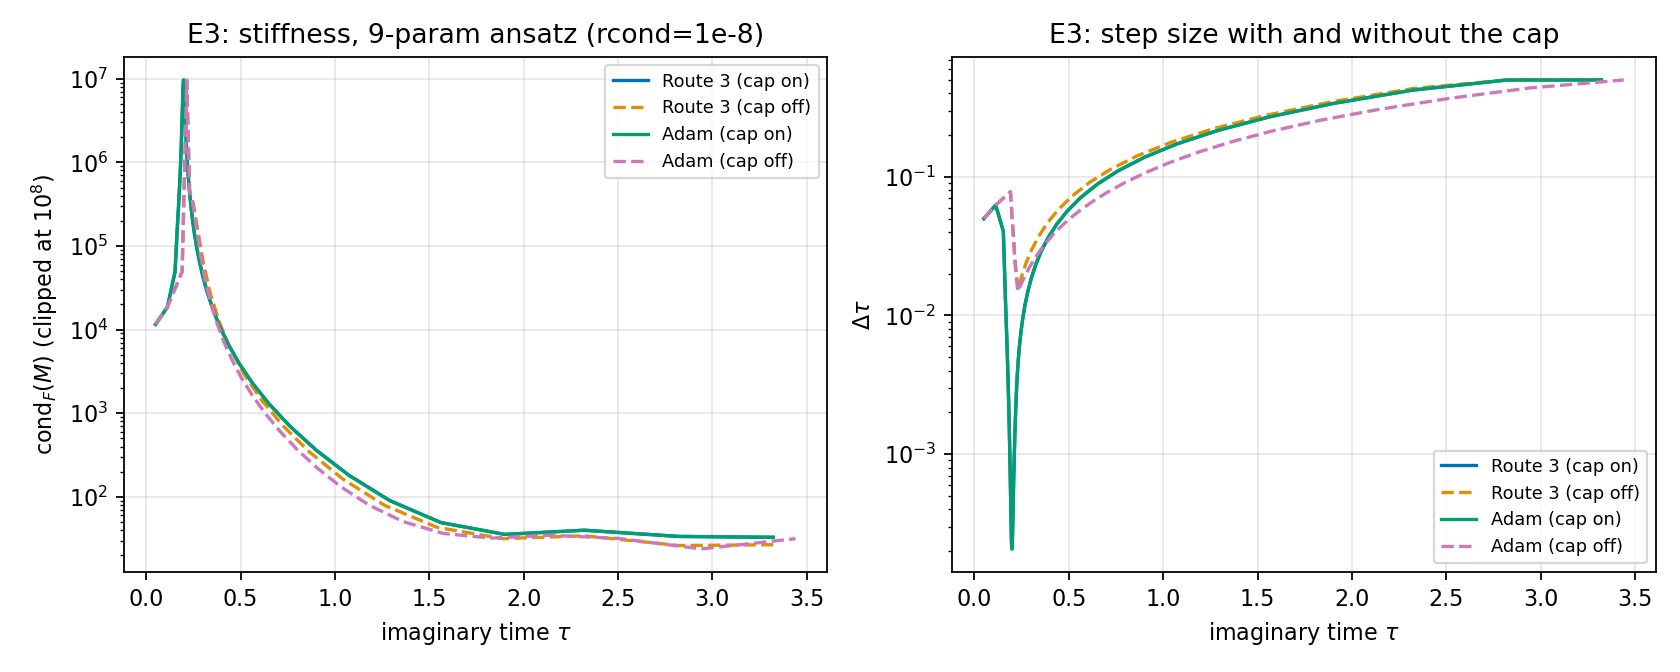
\includegraphics[width=0.8\textwidth]{target_e3_stiffness}
\caption{E3, 9-parameter ansatz at $\rcond=10^{-8}$. Left: $\cond_F(M)$ along the four runs.
It peaks near $10^7$ at $\tau\approx0.2$. Right: step size with and without the cap. With the
cap on, both controllers follow the same trajectory: $\dt$ drops to about $2\times10^{-4}$ at
the peak and recovers afterwards.}
\label{fig:e3}
\end{figure*}

\paragraph*{E1 off-by-one.} The 732-circuit read-out was off by one evaluation. Corrected, the
values are $-1.120983$ against $-1.120952$, and the Adam--Route~3 gap changes from
$+3.5\times10^{-5}$ to $+3.0\times10^{-5}$. The correction is small: the gap between adaptive
and fixed-step control at the same budget is $925\times$ the size of this correction. At this early budget Adam is marginally ahead; read at Route~3's completion budget (Table~\ref{tab:g2}) the order reverses.

\paragraph*{G1, G7.} A broken import left by a folder move was fixed (G1). Latent defects were
recorded (G7), including a hard-coded SHRINK and a plot axis that clips the $s_e=1.015$
excursion.

\subsection{Confirmed positive result: a zero-cost error estimator (G5)}
\label{sec:g5}

The gate already computes $\Delta E_a-\Delta E_p$. Because $Y=-\nabla E$
(Eq.~\eqref{eq:Ygrad}), $\Delta E_p=(\nabla E\cdot\thetadot)\dt$ is the \emph{exact}
first-order Taylor term of $E(\theta+\dt\,\thetadot)$. The discrepancy is therefore a
second-order, local-truncation-error estimate. It costs no extra circuits, whereas an embedded
pair or step doubling needs three additional $f$ evaluations per step. The audit tested this
against step doubling (one full step against two half-steps with a fresh midpoint evaluation)
on the E1 trajectory:
\begin{itemize}
\setlength\itemsep{0pt}
\item first 40 accepted steps: log-Pearson $0.9902$, Spearman $0.9882$; ratio
  $|\Delta E_a-\Delta E_p|/e_{\mathrm{doubling}}$ with median $2.060$ and range
  $[0.350,\,11.439]$;
\item 20 probes: $0.9701$ / median $2.157$; 60 probes: $0.9948$ / $2.026$; all 190 steps:
  $0.9983$ / $2.005$.
\end{itemize}
The expected ratio is exactly~2. If the full-step error is $C\dt^2$, two half-steps incur
$2C(\dt/2)^2=C\dt^2/2$, so step doubling measures $C\dt^2/2$ while $|\Delta E_a-\Delta E_p|$
measures $C\dt^2$ (Appendix~\ref{app:ratio2}). The ratio settles at $2.03$--$2.09$ over the
converged tail.

\paragraph*{Where it fails.} The ratio departs from~2 on a handful of steps (up to $11.4$). The
audit had predicted that these outliers would track the \emph{change} of $\cond(M)$ along the
step, since the estimator does not see the $\partial_\theta M^{+}$ term of $\ddot\theta$. This
prediction \emph{failed}. The correlation of the ratio with the level of $\cond(M)$ is
$-0.8938$, against $+0.3176$ with its change, and the partial correlations are $-0.5437$ and
$+0.1523$. The blind spot exists, but its predicted form does not.

%% ===========================================================================
\section{Phase III: Route-3 controller and its audit}
\label{sec:phase3}

\paragraph*{Question.} Does the memo's Route~3 (Sec.~\ref{sec:baseline}) work on the benchmark,
and what do its indicators actually measure? The implementation defines four targets. Target A
is noiseless convergence on the 5-parameter ansatz. Target B is debiasing under noise. Target
C is stiffness on the 9-parameter ansatz. Target D is a noise-floor scan.

\subsection{Audit (F1--F12)}

The first write-up was audited against live code. The audit
recorded twelve findings (F1--F12) and implemented six correction modules (M1--M6). The
findings that changed results were:
\begin{itemize}
\setlength\itemsep{0pt}
\item F1: the debiasing used the Theorem-2 factor $q^{-1}$ instead of the hardware factor of
  Eq.~\eqref{eq:factor2}.
\item F3: a reported per-step number had no code path that produced it.
\item F4: the RMS trajectory metric extrapolated stalled runs.
\item F5: the energy gate tested against the exact-ITE model instead of the variational
  prediction.
\item F7: Targets B and D shared one random stream, so two runs claimed to be ``identical''
  started from different $\theta_0$.
\item F8, F9: rejected steps were committed, and comparisons were not budget-matched.
\item F10: $\cond(M)$ was read through the regularizer.
\item F12: a term of Eq.~\eqref{eq:Y} was dropped silently. The term vanishes for pure states,
  and this is documented and tested in the post-audit code.
\end{itemize}
The remaining findings concerned naming and code structure. F2 was the label ``flow-direction
error'' for what is a pure magnitude rescaling, F6 a ``zero violations'' claim narrower than
stated, and F11 a duplicated physics layer. All numbers below are post-audit.

\subsection{Target A: convergence and cost}

\begin{figure}[t]
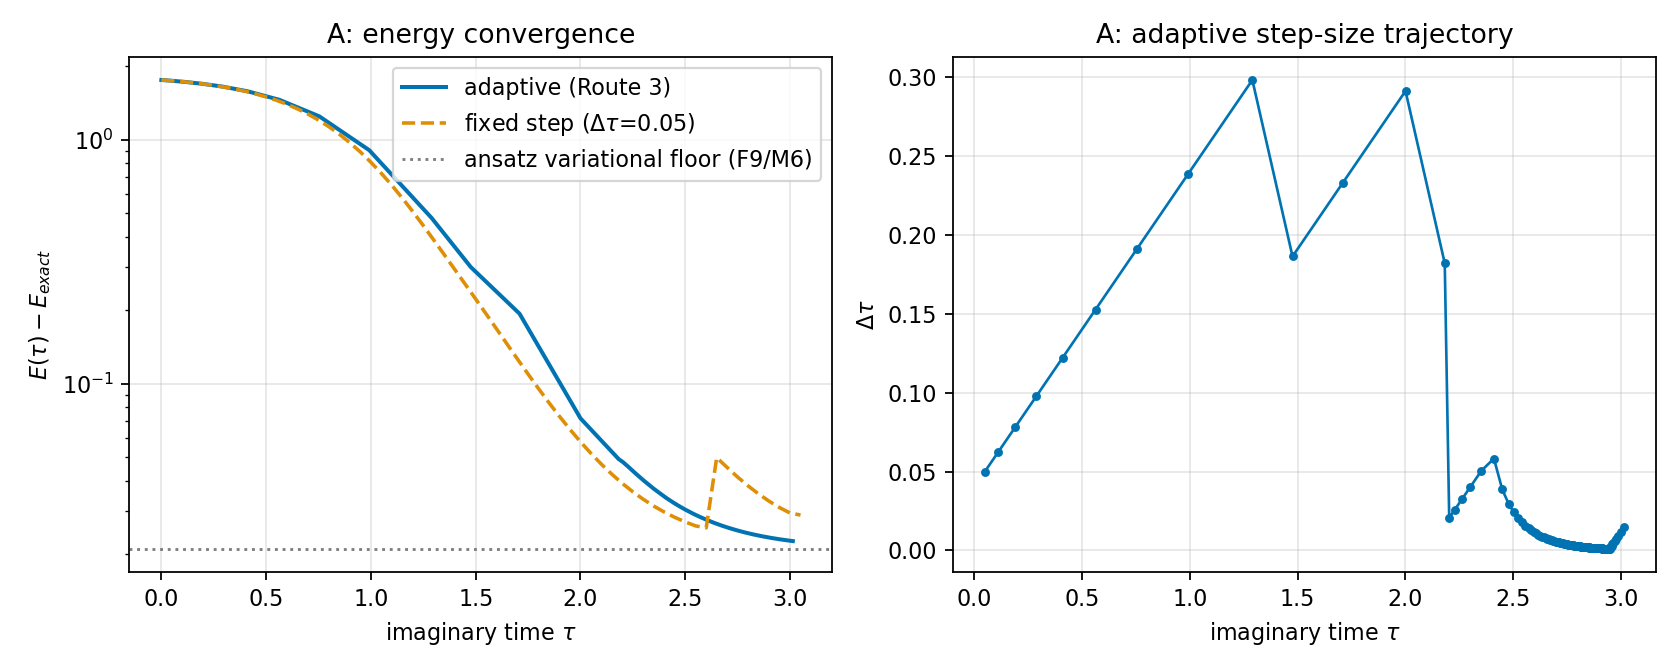
\includegraphics[width=\columnwidth]{target_a_convergence}
\caption{Target A: Route~3 against fixed-step Euler on the noiseless 5-parameter ansatz.}
\label{fig:targetA}
\end{figure}

Route~3 reaches $E=-1.122993$ in 172 steps (Fig.~\ref{fig:targetA}). The fair comparison is at equal circuit count. At 732 circuits it is at $-1.120952$ (the corrected read-out of Sec.~\ref{sec:phase2}), which is $3.648\times10^{-3}$ above $\Efloor$, while
fixed-step Euler is at $-1.116691$, $7.909\times10^{-3}$ above. That is $2.2\times$ closer to the floor; both gaps are differences of pinned energies. Run to completion, Route~3 ends $1.607\times10^{-3}$ above $\Efloor$ after 2069 circuits, $5\times$ closer than Euler's end point but at $2.8\times$ its cost. Of the 2069 circuits, 1892 went to $f$ evaluations and 177 to energy-gate trials (172 first trials and 5 retries, on 3 steps). Over the last 43 steps the cap binds
on 31 and the gate retries on 0. The step collapse near $\tau_{\max}$ is therefore the
stiffness cap, not the gate. Over the same steps $\sigma_{\min}$ ranges over
$[3.464\times10^{-7},\,1.804\times10^{-2}]$ and the unregularized spectral $\cond(M)$ over
$[32.61,\,1.445\times10^6]$. The pre-audit comparison ($-1.1197$ against $-1.1167$ at 61
evaluations) is superseded.

\subsection{Target B: debiasing under noise}

With the corrected factor (Eq.~\eqref{eq:factor2}), the debiased flow matches the clean flow to
the finite-difference floor at every $p$ (Fig.~\ref{fig:targetB}). The per-step error is $0.00000\%$, against $5.31458\%$
(biased) at $p=0.02$ and $34.67544\%$ at $p=0.1$. The noisy flow is exactly collinear with the
clean one. The collinearity residuals are $1.882\times10^{-8}$ and $1.403\times10^{-8}$, and the
measured scale factor equals the closed form $c(p)=1+(1-q)/(2q)$ to six digits ($1.053146$ and
$1.346754$). Over full trajectories, however, debiasing gives no consistent advantage. The RMS
deviations from the noiseless run are $1.254\times10^{-1}$ (debiased) against
$1.228\times10^{-1}$ (biased) at $p=0.02$, and $5.356\times10^{-1}$ against
$5.314\times10^{-1}$ at $p=0.1$.

The reason is structural. A scalar rescaling $\thetadot\to c\,\thetadot$ is indistinguishable,
for any controller that is homogeneous in $\thetadot$, from a faster flow, so an adaptive
controller partly absorbs it as a reparametrization of $\tau$. A single test supports this
reading. The noiseless controller with every $\dt$ divided by $c(p)$ tracks the biased run
better than the plain baseline does (RMS $11.9\%$ against $12.5\%$ at $p=0.02$; $35.2\%$ against
$50.6\%$ at $p=0.1$). This test was run once and has no committed code path. The pre-audit
``surprise'' of a per-step debiasing error growing from about 5\% to about 67\% was produced by
the wrong factor, and it is retracted.

\begin{figure}[t]
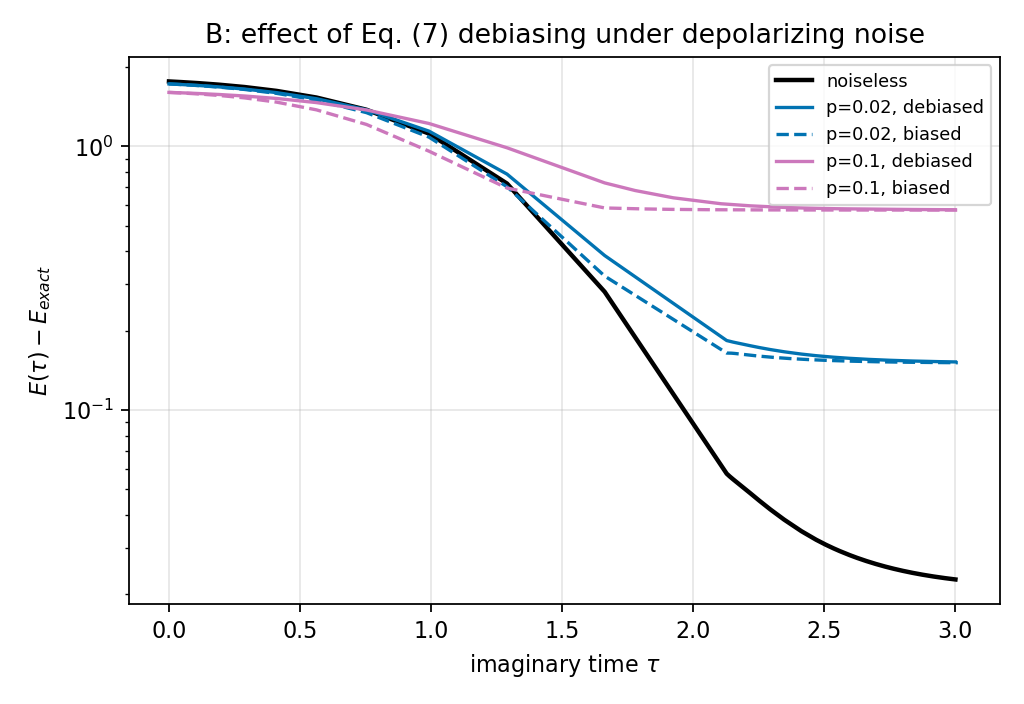
\includegraphics[width=\columnwidth]{target_b_debiasing}
\caption{Target B: energy above the exact ground state for the noiseless run and for
debiased (solid) and biased (dashed) runs at $p=0.02$ and $p=0.1$. Both noisy pairs saturate
well above the noiseless trajectory, and debiasing does not bring them systematically closer
to it.}
\label{fig:targetB}
\end{figure}

\subsection{Target C: the cutoff is part of the method}

On the rank-6 9-parameter ansatz, the tight cutoff $\rcond=10^{-8}$ reaches an error of
$8.9\times10^{-4}$ in 108 steps. Along the way $\cond(M)$ ranges over
$[32.9,\,9.66\times10^6]$ and $\dt$ over $[2.07\times10^{-4},\,0.5]$. The loose cutoff
$10^{-2}$ reaches $2.1\times10^{-3}$ in 17 steps, with $\cond(M)$ in $[19.1,\,125]$ and $\dt$
in $[0.05,\,0.5]$. The tight cutoff wins by $2.4\times$ in final error (Fig.~\ref{fig:targetC}). A lower reported
$\cond(M)$ does not mean a better solve, and it is wrong to report $\cond(M)$ without its
cutoff. Before the gate fix the same runs gave 20 steps / $1.2\times10^{-2}$ and a 500-step
stall / $2.9\times10^{-2}$. Most of that earlier gap came from the broken gate.

\begin{figure}[t]
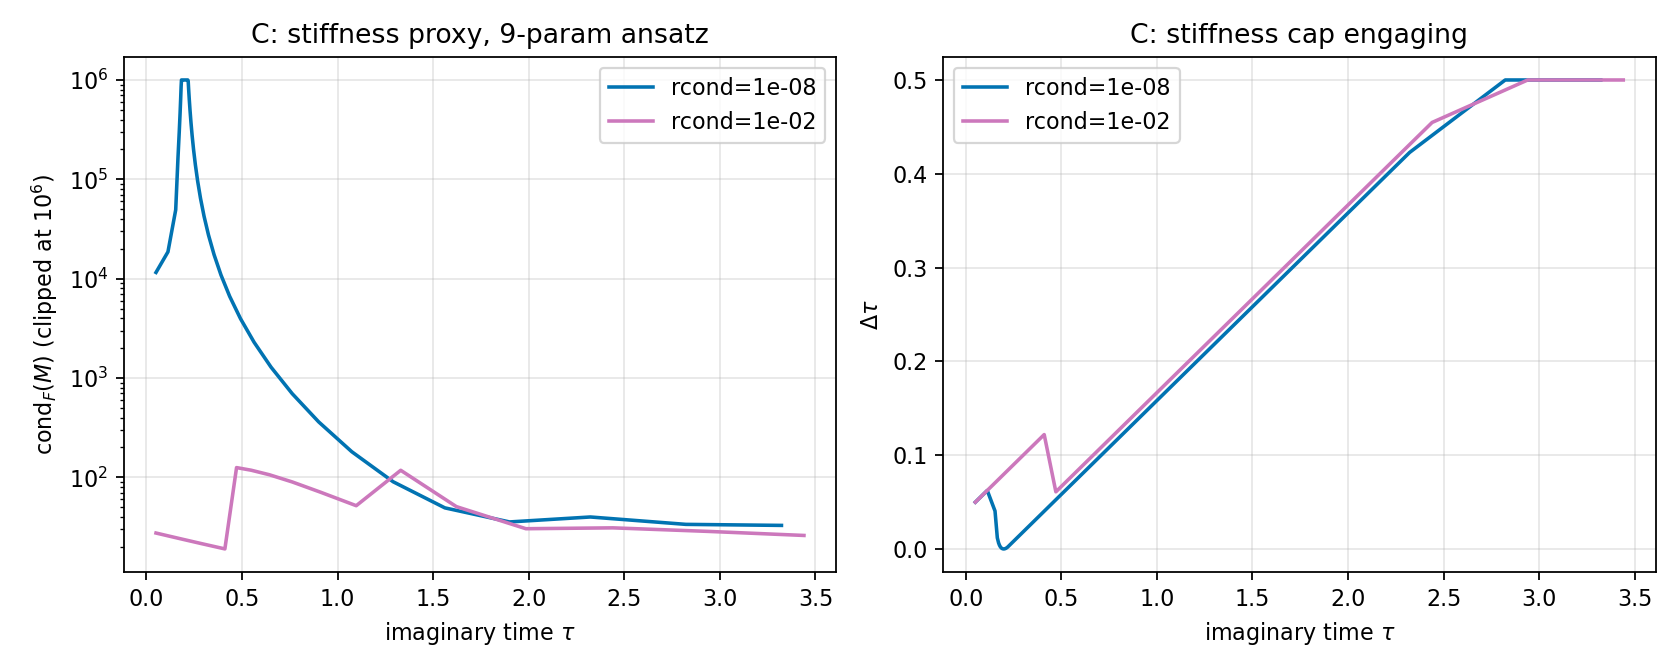
\includegraphics[width=\columnwidth]{target_c_stiffness}
\caption{Target C, 9-parameter ansatz. Left: $\cond_F(M)$ (clipped at $10^6$) for
$\rcond=10^{-8}$ and $10^{-2}$. The loose cutoff hides the peak near $\tau\approx0.2$. Right:
step size. At the tight cutoff the stiffness cap drives $\dt$ down at the peak, and both runs
then grow to $\dt_{\max}$.}
\label{fig:targetC}
\end{figure}

\subsection{Target D: no noise floor}

Table~\ref{tab:targetD} shows the RMS energy deviation from the noiseless run as a function of
$p$. It grows smoothly and roughly linearly, with no knee. The pre-audit reading of a
floor-like feature near $p\approx10^{-3}$ rested on the stall-contaminated metric (F4) and
the wrong factor (F1), and it is retracted.

\begin{table}[t]
\caption{Target D: RMS energy deviation from the noiseless trajectory.}
\label{tab:targetD}
\begin{ruledtabular}
\begin{tabular}{lll}
$p$ & debiased & biased \\
\midrule
$10^{-4}$ & $6.376\times10^{-4}$ & $6.067\times10^{-4}$ \\
$10^{-3}$ & $6.365\times10^{-3}$ & $6.051\times10^{-3}$ \\
$10^{-2}$ & $6.253\times10^{-2}$ & $5.992\times10^{-2}$ \\
$5\times10^{-2}$ & $2.884\times10^{-1}$ & $2.762\times10^{-1}$ \\
\end{tabular}
\end{ruledtabular}
\end{table}

%% ===========================================================================
\section{Phase IV: replication of variational product formulas}
\label{sec:phase4}

\paragraph*{Why this paper.} Assi \emph{et al.}~\cite{BeyondTrot2026} evolve in \emph{real} time
with a variational product formula. The parameters (exponent coefficients) obey a
McLachlan-type equation with a metric $g$ that plays the same role as $M$ here. The ansatz
contains repeated exponentials, so $g$ is singular at $t=0$ and the method needs a starting
time $t_0>0$. This is a second, independent instance of the degeneracy faced by the controllers studied here.
Table~\ref{tab:bt} gives the verdicts.

\begin{table*}[t]
\caption{Phase IV verdicts for Ref.~\cite{BeyondTrot2026}. ``QIM'' is the quantum Ising model
with $N=5$ used in the paper. Read-off precision from figures is $\pm0.001$.}
\label{tab:bt}
\begin{ruledtabular}
\begin{tabular}{p{6.4cm}p{3.6cm}p{3.6cm}l}
Target & Paper & This work & Verdict \\
\midrule
T1 gate counts, $N=2$--$12$ & $R_x=2N$, $R_z=4N-2$, CNOT $4N-4$ & identical & \verdict{reproduced} \\
T1 circuit vs \texttt{expm}, computed angles / Fig.~12 angles & exact & $2.8\times10^{-16}$ / $1.7286$ & \verdict{reproduced} / \verdict{not} \\
T2 two-level model, Eqs.~(31)--(36) & exact & $\le2.8\times10^{-14}$ & \verdict{reproduced} \\
T2$'$ Fig.~2(b) error floor & ``of order $10^{-7}$'' & $4.0\times10^{-11}$ & inconclusive \\
T3 $\mathcal E_F(t{=}1)$, four curves of Fig.~4(a) & 0.0212, 0.0212, 0.0692, 0.0514 & 0.021217, 0.021143, 0.068847, 0.052034 & \verdict{reproduced} ($\le1.23\%$) \\
T3$'$ same, as stated in the text & 1.5\% / 3\% & 0.0211 / 0.0688 & \verdict{not reproduced} \\
T3$''$ variational beats Ruth on all of $[0,2]$ & true & false & \verdict{not reproduced} \\
T4 Eq.~(61)$\to$(69), labels as printed / $A\leftrightarrow B$ & exact & $2.2334$ / $3.6\times10^{-16}$ & \verdict{not} / \verdict{reproduced} \\
T4 Fig.~13 at $t=100$, raw norm & 0.2694, 0.1715 & 0.26951, 0.171821 & \verdict{reproduced} \\
T4 same, normalized by Eq.~(27) & 0.2694, 0.1715 & 0.023822, 0.015187 & \verdict{not reproduced} \\
T5 Eq.~(65)$=$(68), printed / $A\leftrightarrow B$ & 15/15 & 0/15 / 15/15 & \verdict{not} / \verdict{reproduced} \\
T5 $\Xi$ predicts the better ordering & 7/7 & 0/7 literal, 7/7 relabelled & only relabelled \\
T7 stroboscopic $\mathcal E_F(t{=}100)$ & 0.11, 0.055 & 0.108968, 0.055305 & \verdict{reproduced} \\
T8 advantage grows with $\tau$ & true & 1 of 3 statistics & \verdict{partially reproduced} \\
\end{tabular}
\end{ruledtabular}
\end{table*}

\paragraph*{The figures reproduce, the text does not.} Figure~4(a) reproduces to within
$1.23\%$ on all four curves, and the Ruth-to-variational ratio at $t=1$ is $2.461$. The text on
the same page quotes $1.5\%$ and $3\%$, which misses the figure by $+41\%$ and $+73$--$129\%$.
The claim that the variational formula beats Ruth's over the \emph{entire} interval is false.
The two errors scale with slopes $2.999$ and $4.999$ in $t$ and cross at $t=0.376$ (bracket
$0.375$--$0.426$). At $t=10^{-3}$ Ruth's formula is better by up to five orders of magnitude.

\paragraph*{Label swap and normalization.} Equations~(61), (65), (68) and (69) use the $A$
and $B$ labels swapped relative to Eq.~(54). As printed, Eq.~(61)$\to$(69) misses by $2.2334$
and the Eq.~(65)$=$(68) check passes on 0 of 15 cases. With the labels swapped, the error is
$3.6\times10^{-16}$ and the check passes on 15 of 15. Figure~13 reproduces with the raw
Frobenius norm but not with the paper's own Eq.~(27) normalization, which differs by
$2\sqrt D=11.3137$.

\paragraph*{T2$'$ is not scorable.} The $10^{-7}$ floor of Fig.~2(b) is set by the integrator
tolerance, which the paper does not state. The maximum error of the replication runs from $9.9\times10^{-4}$ at
$\texttt{rtol}=10^{-3}$ down to $3.3\times10^{-13}$ at $10^{-12}$, and is $4.0\times10^{-11}$ at
the tolerance fixed before the run. A floor of $10^{-7}$ corresponds to an
$\texttt{rtol}$ between $10^{-8}$ and $10^{-6}$. The number reflects the authors' integrator
settings and says nothing about the method.

\paragraph*{New result: $\cond(g)$ and its boundary layer (T6).} The paper never reports
$\cond(g)$, even though the method inverts $g$ at every step. For the two-level metric of
Eq.~(35), $\cond(g)$ depends only on the first coefficient $c_1$ (Table~\ref{tab:condg}). At
$c_1=0$ the matrix drops to rank~2 of~3 with null vector $\propto(1,0,-1)$, because the two
$A$ exponentials of the ABA ansatz become indistinguishable. For $c_1\in[10^{-6},10^{-3}]$ the
fitted exponent is $\cond(g)\propto c_1^{-2.0000}$. Along the QIM trajectory $\cond(g)$ starts
at $3.4\times10^{12}$ (BAB) and $2.1\times10^{16}$ (ABAB) and falls to $1.36$ and $4.85$ at $t=2$
(Fig.~\ref{fig:condg}). The ill-conditioning is real but confined to a boundary layer, and
the result is insensitive to how it is regularized. Varying $t_0\in[10^{-8},10^{-3}]$ and
$\rcond\in[10^{-14},10^{-4}]$ moves $\mathcal E_F(t{=}2)$ by at most $5.12\times10^{-10}$
relative.

\begin{table}[t]
\caption{T6: conditioning of the two-level metric $g$ of Ref.~\cite{BeyondTrot2026}, Eq.~(35).}
\label{tab:condg}
\begin{ruledtabular}
\begin{tabular}{llcl}
$c_1$ & $\det g$ & rank & $\cond(g)$ \\
\midrule
0 & 0 & 2 of 3 & $2.2\times10^{17}$ \\
$10^{-6}$ & $4.0\times10^{-8}$ & 3 & $2.50\times10^{11}$ \\
$10^{-3}$ & $4.0\times10^{-2}$ & 3 & $2.50\times10^{5}$ \\
0.2 & $1.2865\times10^{3}$ & 3 & 10.60 \\
\end{tabular}
\end{ruledtabular}
\end{table}

\begin{figure}[t]
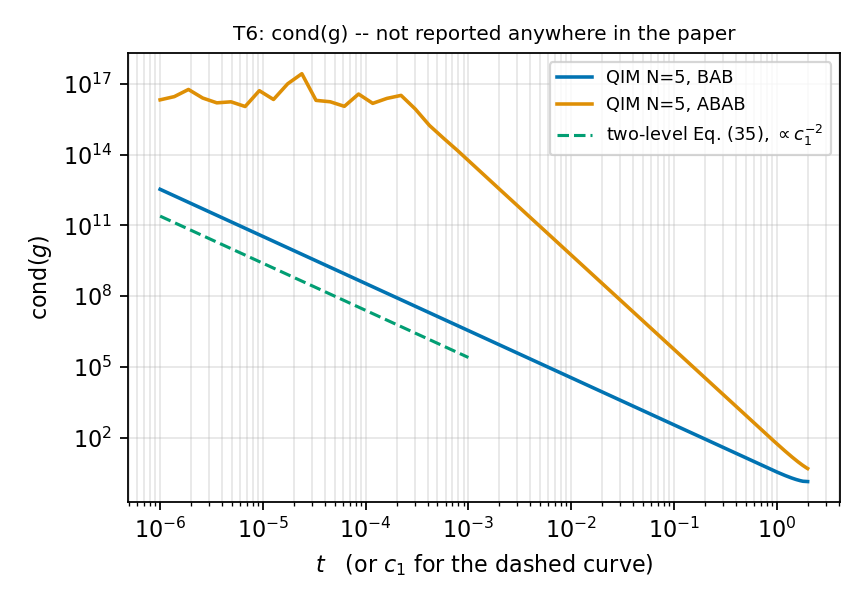
\includegraphics[width=\columnwidth]{cond_g_trajectory}
\caption{T6: $\cond(g)$ along the QIM ($N=5$) trajectory for the BAB and ABAB ansätze, and the
two-level closed form (dashed, against $c_1$), which scales as $c_1^{-2}$.}
\label{fig:condg}
\end{figure}

%% ===========================================================================
\section{Phase V: pre-registered experiments P1 and P2}
\label{sec:phase5}

Phase~V consists of two experiments, each with written predictions registered before it was
run. P1 asks what the $\cond(M)\sim10^7$ events of Target~C and E3 are. P2 asks whether a
step law with an explicit tolerance controls the achieved error.

\subsection{P1: classifying the singularity}

\paragraph*{Hypotheses.} The large $\cond(M)$ could come from (a) gauge leakage, meaning the
three structural null directions of the rank-6 metric passing the cutoff, (b)
finite-difference noise in $M$, or (c) a genuine singularity of the parametrization.

\paragraph*{Predictions and outcome.} Table~\ref{tab:p1score} scores the predictions.
\begin{table}[t]
\caption{P1 scorecard.}
\label{tab:p1score}
\begin{ruledtabular}
\begin{tabular}{p{4.6cm}l}
Registered prediction & Outcome \\
\midrule
$\sigma_{7\text{--}9}$ below the $10^{-8}\sigma_1$ cutoff (no leakage) & held \\
$\sigma_{7\text{--}9}$ at $10^{-10}$--$10^{-12}$ & failed (favourably) \\
rank-6 $\cond$ equals logged $\cond$ along E3 & held \\
the cap reads real stiffness & held \\
the soft mode is a near-degenerate gate \emph{pair} & failed \\
\end{tabular}
\end{ruledtabular}
\end{table}

\paragraph*{No gauge leakage.} The largest $\sigma_7/\sigma_1$ is $2.021\times10^{-16}$ at
$\rcond=10^{-8}$ and $1.321\times10^{-16}$ at $10^{-2}$. At $10^{-8}$ the pseudo-inverse always
keeps exactly 6 modes. At $10^{-2}$ it keeps 4 to 6, and fewer than 6 on 11 of 17 steps. The
rank-6 condition number equals the logged value to $1.11\times10^{-15}$. The gauge singular
values sit lower than predicted because $M$ is a Gram matrix. A true null vector picks up a
contribution that is \emph{second} order in the finite-difference error, about $10^{-20}$,
so what remains is the eigensolver's roundoff at about $10^{-16}$. The per-entry error
$\max|M_{\mathrm{fd}}-M_{\mathrm{exact}}|$ is $1.652\times10^{-10}$ ($1.715\times10^{-10}$ at the
loose cutoff).

\paragraph*{Identities.} The state form Eq.~\eqref{eq:stateform} agrees with the finite
differences to $2.594\times10^{-10}$ for $M$ and $3.955\times10^{-10}$ for $Y$. The opposite sign
convention gives $1.589$, so the sign is fixed unambiguously. The CRZ row of $M$ is exactly zero
at $\theta=0$, and Eq.~B9 of Ref.~\cite{QDP2024} holds to $7.216\times10^{-16}$.

\paragraph*{A chart singularity.} The peak is at step 43, $\tau=0.1983$, with singular values
\begin{multline*}
[0.9991,\,0.9828,\,0.1463,\,0.09246,\,0.02142,\,1.461{\times}10^{-7},\\
1.4{\times}10^{-16},\,3.3{\times}10^{-17},\,8.8{\times}10^{-19}].
\end{multline*}
The soft mode $v_6$ loads on a single gate (th8, weight $+0.934$; th3 $+0.233$, th2
$-0.172$). At this point $\langle Z_0\rangle=0.9944$ and $M_{88}=5.568\times10^{-3}$. The gates
pair up in the \emph{gauge} vectors instead (Fig.~\ref{fig:p1null}): $v_7=$ th1$-$th6 ($\mp0.693$), $v_8\approx$
th2$-$th7 ($+0.638/-0.609$), $v_9\approx$ th4 ($-0.998$). Table~\ref{tab:p1speed} and Fig.~\ref{fig:p1} are the
decisive evidence. Near the peak the parameter speed $\|\thetadot\|$ grows by two orders of
magnitude, and almost all of it lies along $v_6$, while the \emph{state} speed $\|\dot\rho\|$
barely moves. Over the whole run $\|\thetadot\|$ varies by a factor of $160.8$ and
$\|\dot\rho\|$ by only $8.83$. The state moves smoothly through a region where the chart
$\theta\mapsto\rho$ folds, so a small state displacement needs a large parameter
displacement. This is a coordinate singularity, and it is real stiffness in the sense relevant to an explicit integrator. The
$\cond(M)$ cap therefore reads a genuine property, and the attribution of E3 to the cap (G6)
is supported. There are 86 of 108 steps with $\cond>10^5$ at $\rcond=10^{-8}$, against 0 of 17
at $10^{-2}$. The largest logged $\cond$ is $9.6637\times10^6$ against $125.39$, and the
largest spectral value $6.8367\times10^6$ against $1.9281\times10^5$.

\begin{table}[t]
\caption{P1: speeds along the E3 trajectory ($\rcond=10^{-8}$). The last column is the
fraction of $\thetadot$ along the soft singular vector $v_6$.}
\label{tab:p1speed}
\begin{ruledtabular}
\begin{tabular}{lllll}
$\tau$ & $\cond$ & $\|\thetadot\|$ & $\|\dot\rho\|$ & along $v_6$ \\
\midrule
0      & $1.156\times10^{4}$ & 0.7989 & 0.1428 & 0.351 \\
0.1880 & $2.492\times10^{6}$ & 35.23  & 0.1826 & 0.99979 \\
0.1949 & $7.392\times10^{6}$ & 98.8   & 0.1848 & 0.999992 \\
0.1983 & $9.664\times10^{6}$ & 128.4  & 0.1862 & 0.9999978 \\
0.2016 & $7.476\times10^{6}$ & 100.2  & 0.1877 & 0.999989 \\
2.8223 & 32.85 & 0.6401 & 0.257 & 0.276 \\
\end{tabular}
\end{ruledtabular}
\end{table}

\begin{figure*}[t]
\centering
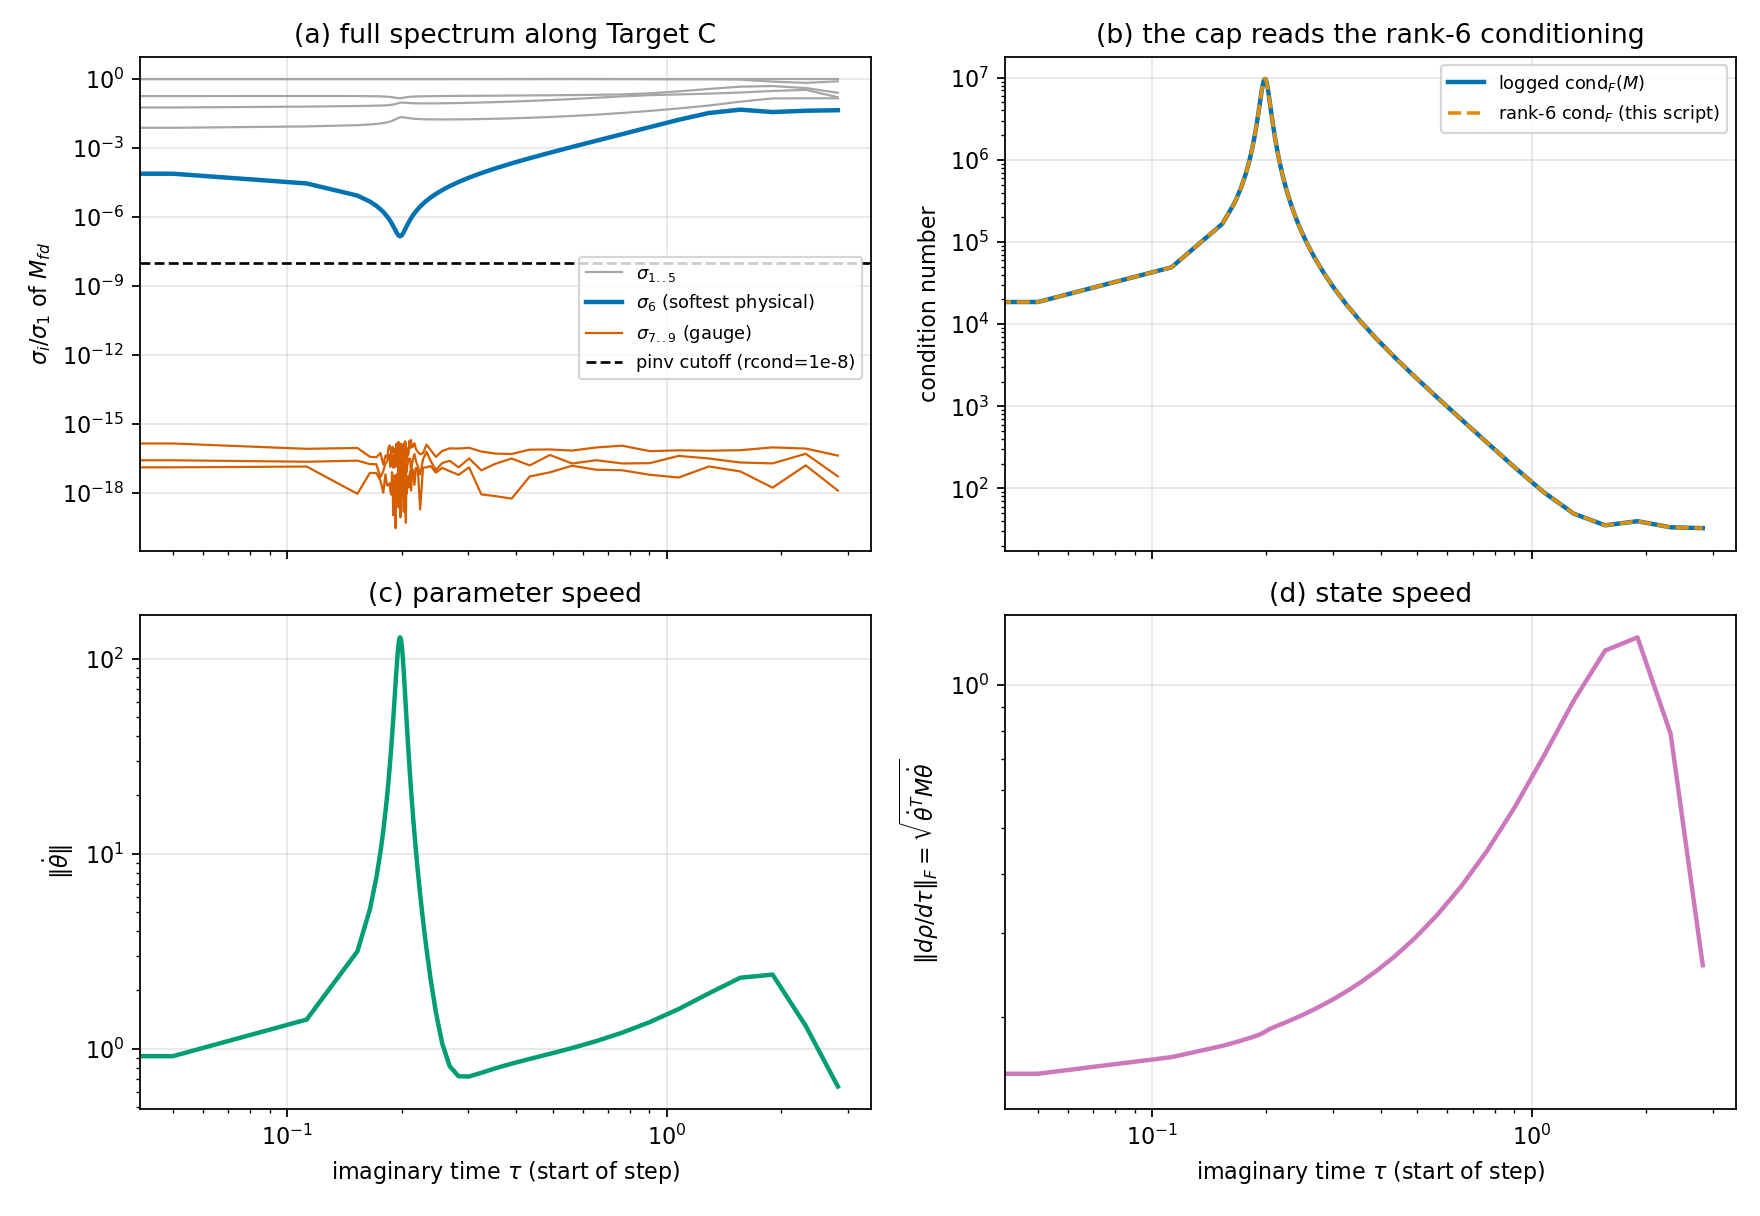
\includegraphics[width=0.78\textwidth]{p1_target_c_spectrum}
\caption{P1, Target~C/E3 run at $\rcond=10^{-8}$. (a) Singular values of $M$ relative to
$\sigma_1$. The three gauge modes stay at roundoff, far below the cutoff (dashed). The soft
physical mode $\sigma_6$ dips to about $10^{-7}$ at $\tau\approx0.2$. (b) The logged
$\cond_F(M)$ and the rank-6 value coincide. (c) The parameter speed spikes at the peak.
(d) The state speed $\|\dot\rho\|_F=\sqrt{\thetadot^{\top}M\thetadot}$ does not.}
\label{fig:p1}
\end{figure*}

\begin{figure}[t]
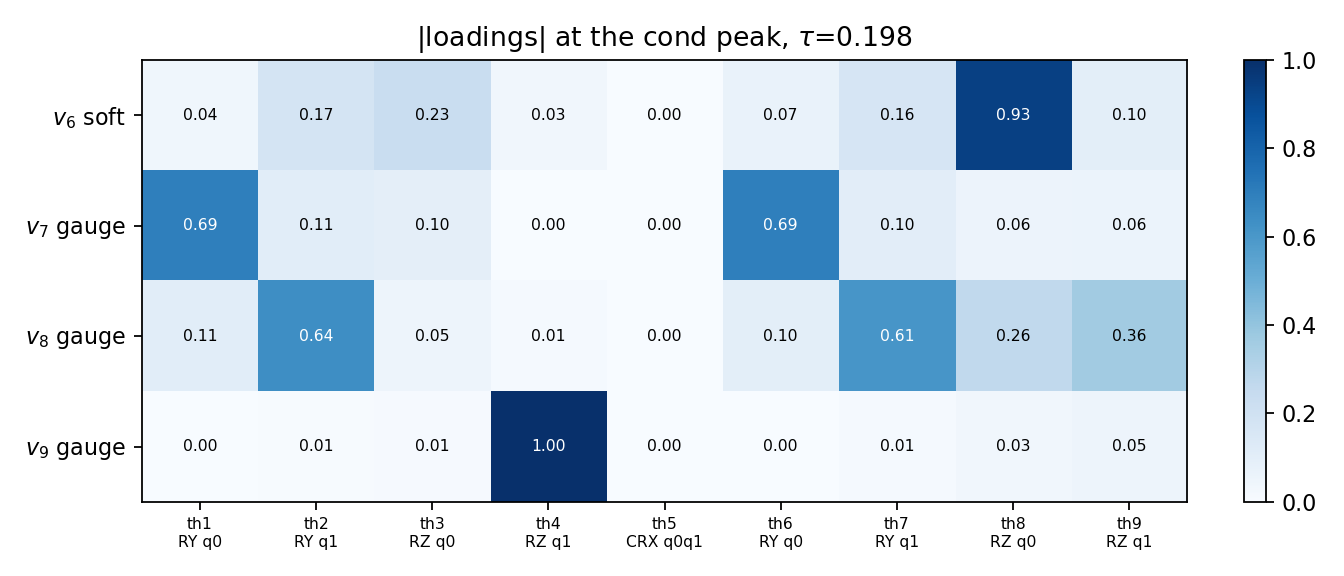
\includegraphics[width=\columnwidth]{p1_null_vectors}
\caption{P1: absolute loadings of the soft vector $v_6$ and the gauge vectors $v_{7\text{--}9}$
on the nine gates at the $\cond$ peak, $\tau=0.198$.}
\label{fig:p1null}
\end{figure}

\paragraph*{The fold amplifies finite-difference error, but only locally.} Re-running with the
exact state-form metric changes almost nothing. At $\rcond=10^{-8}$ the final error is
$8.868181\times10^{-4}$ (finite differences) against $8.854194\times10^{-4}$ (exact), both in
108 steps, with largest $\cond$ $9.66375\times10^6$ against $9.66367\times10^6$. At $10^{-2}$
both runs give $2.143405\times10^{-3}$. The energy gap between the two runs is
$1.292\times10^{-11}$ before the fold. It peaks at $1.101\times10^{-4}$ ($\tau=2.3223$) and ends
at $6.068\times10^{-6}$. At the loose cutoff the gap stays at or below $1.228\times10^{-9}$.

\paragraph*{A second mechanism on the 5-parameter ansatz.} As a control, Target~A (error
$2.2606\times10^{-2}$ in 172 steps) keeps only 4 modes on 12 of 172 steps, all in
$\tau\in[2.945,\,2.999]$. There the soft vector is the CRZ gate alone ($+0.999$) with
$\sigma_5/\sigma_1=6.921\times10^{-7}$ at $\tau=2.9987$. The state is almost a computational
basis state, with populations $7.53\times10^{-4}$, $1.74\times10^{-7}$, $0.99902$ and
$2.30\times10^{-4}$ and $\langle Z_1\rangle=0.99954$. A controlled rotation whose control qubit
is almost deterministic has almost zero generator variance, so its metric entry vanishes
($M_{\mathrm{CRZ}}=8.3662\times10^{-4}$). This is a zero-variance mechanism, distinct from the
fold. $\|\thetadot\|$ varies by $116.7\times$ here.

\paragraph*{A regime-aware cap is rejected.} Feeding the cap the rank-6 condition number
instead of the logged one was tested (Table~\ref{tab:p1cap}). At the tight cutoff it changes
nothing. At the loose cutoff it makes the cap bind on 67 steps where it bound on none, and
the error rises from $2.1434\times10^{-3}$ to $3.4051\times10^{-3}$. The variant was rejected.

\begin{table}[t]
\caption{P1: cap fed by the logged or the rank-6 $\cond$.}
\label{tab:p1cap}
\begin{ruledtabular}
\begin{tabular}{lllrr}
\rcond & cap reads & error & steps & binding \\
\midrule
$10^{-8}$ & logged & $8.8682\times10^{-4}$ & 108 & 82 \\
$10^{-8}$ & rank-6 & $8.8617\times10^{-4}$ & 108 & 82 \\
$10^{-2}$ & logged & $2.1434\times10^{-3}$ & 17  & 0 \\
$10^{-2}$ & rank-6 & $3.4051\times10^{-3}$ & 105 & 67 \\
\end{tabular}
\end{ruledtabular}
\end{table}

\subsection{P2: does the achieved error track a requested tolerance?}

\paragraph*{Set-up.} Neither controller of Phases~II--III has a tolerance to sweep. Route~3
ratchets, and Adam's setpoint is the reject band (G4). P2 therefore drives the step with the
PI law Eq.~\eqref{eq:PI} ($k_I=0.15$, $k_P=0.2$), fed by the zero-cost estimator of
Sec.~\ref{sec:g5}, $e_n=|\Delta E_a-\Delta E_p|/2$. The reject band stays as the gate. Two
error-per-step policies are compared: EPS ($e_n\le\tol$) and EPUS ($e_n/\dt\le\tol$). For an
order-1 method they predict end-point error $\propto\tol^{1/2}$ and $\propto\tol^{1}$
respectively (Appendix~\ref{app:eps}). The reference is an exact-metric DOP853 solution at
$\texttt{rtol}=10^{-11}$, with self-check $8.25\times10^{-12}$. A run qualified for the fit
only if all of the following held, as registered in advance: it exits at $\tau_{\max}$, the
cap binds on fewer than 25\% of steps, $\dt$ sits at a bound on fewer than 25\% of steps, and
the error is more than $10\times$ the reference floor. At least three qualifying runs were
required.

\paragraph*{Outcome.} Only 2 of 9 EPS runs and 2 of 8 EPUS runs qualified, so no exponent
could be fitted. Five of the six registered predictions (the three exponent windows, the
location of the break, and the circuit slope) therefore score as \emph{failed for lack of a
fit}. None of them failed because a slope was measured outside its window. The prediction
that did hold is the one that tests G4: with a tolerance separate from the band, growth $<1$
occurs in every run (527 of 1234 steps at EPS $\tol=10^{-6}$). Where $\tol$ lies below the
estimator's natural scale, the median of $e_n/\tol$ is $0.99$. The PI law does control
$e_n$. It is the end-point error that fails to follow.

\begin{table*}[t]
\caption{P2 tolerance sweeps. ``err'' is $|E(\tau_{\mathrm{end}})-E_{\mathrm{ref}}|$; ``max err''
is the maximum along the run; ``cap'' is the fraction of steps on which the stiffness cap binds;
``shrink'' counts steps with growth $<1$; the last column is the median of $e_n/\tol$.
Qualifying runs are the first two of each arm.}
\label{tab:p2}
\begin{ruledtabular}
\begin{tabular}{lllrrrrl}
Arm & $\tol$ & err$(\tau_{\mathrm{end}})$ & max err & steps & circuits & cap\,\% & shrink / med.\ $e_n/\tol$ \\
\midrule
EPS & $10^{-6}$ & $1.1067\times10^{-5}$ & $6.977\times10^{-3}$ & 1234 & 14808 & 10.8 & 527 / 0.992 \\
    & $3.16\times10^{-6}$ & $1.9022\times10^{-5}$ & $9.066\times10^{-3}$ & 761 & 9132 & 18.4 & 295 / 0.974 \\
    & $10^{-5}$ & $2.5242\times10^{-5}$ & $1.291\times10^{-2}$ & 497 & 5964 & 29.0 & 163 / 0.897 \\
    & $3.16\times10^{-5}$ & $2.3316\times10^{-5}$ & $1.917\times10^{-2}$ & 351 & 4212 & 41.6 & 91 / 0.775 \\
    & $10^{-4}$ & $1.4299\times10^{-5}$ & $2.918\times10^{-2}$ & 270 & 3240 & 54.4 & 52 / $3.35\times10^{-3}$ \\
    & $3.16\times10^{-4}$ & $5.6702\times10^{-6}$ & $4.468\times10^{-2}$ & 225 & 2700 & 65.3 & 29 / $2.61\times10^{-4}$ \\
    & $10^{-3}$ & $3.6387\times10^{-5}$ & $6.479\times10^{-2}$ & 200 & 2400 & 73.5 & 14 / $4.75\times10^{-5}$ \\
    & $3.16\times10^{-3}$ & $4.2490\times10^{-4}$ & $8.954\times10^{-2}$ & 184 & 2208 & 79.9 & 6 / $9.5\times10^{-6}$ \\
    & $10^{-2}$ & $2.5438\times10^{-4}$ & $1.130\times10^{-1}$ & 180 & 2162 & 80.0 & 2 / $2.9\times10^{-6}$ \\
\midrule
EPUS & $3.16\times10^{-4}$ & $2.9473\times10^{-5}$ & $8.413\times10^{-3}$ & 2260 & 27120 & 6.2 & 1110 / 1 \\
     & $10^{-3}$ & $3.0816\times10^{-5}$ & $1.420\times10^{-2}$ & 822 & 9864 & 17.8 & 339 / 0.985 \\
     & $3.16\times10^{-3}$ & $2.4532\times10^{-5}$ & $2.751\times10^{-2}$ & 371 & 4452 & 39.6 & 105 / 0.633 \\
     & $10^{-2}$ & $1.1781\times10^{-5}$ & $5.366\times10^{-2}$ & 228 & 2736 & 64.9 & 30 / $2.43\times10^{-3}$ \\
     & $3.16\times10^{-2}$ & $2.4098\times10^{-4}$ & $8.966\times10^{-2}$ & 186 & 2233 & 78.0 & 7 / $4.07\times10^{-4}$ \\
     & $0.1$ & $4.7659\times10^{-4}$ & $1.209\times10^{-1}$ & 176 & 2115 & 81.8 & 2 / $1.08\times10^{-4}$ \\
     & $0.316$ & $7.0607\times10^{-4}$ & $1.325\times10^{-1}$ & 172 & 2068 & 83.1 & 2 / $3.23\times10^{-5}$ \\
     & $1$ & $2.4412\times10^{-3}$ & $1.325\times10^{-1}$ & 56 & 676 & 67.9 & 1 / $1.67\times10^{-4}$ \\
\end{tabular}
\end{ruledtabular}
\end{table*}

Table~\ref{tab:p2} and Fig.~\ref{fig:p2} give the full sweeps. The local slopes of $\log\mathrm{err}$ against
$\log\tol$ between neighbouring runs wander from $-0.80$ to $+2.62$: $+0.47$, $+0.25$, $-0.07$,
$-0.42$, $-0.80$, $+1.61$, $+2.13$, $-0.45$ for EPS and $+0.04$, $-0.20$, $-0.64$, $+2.62$, $+0.59$,
$+0.34$, $+1.08$ for EPUS. The cap takes over at $\tol=10^{-5}$ (EPS) and $3.16\times10^{-3}$
(EPUS), with first binding between $\tau=2.091$ and $2.409$. For reference, under the same
metric Route~3 ends at $6.3181\times10^{-4}$ (172 steps, 2069 circuits) and Adam at
$7.2773\times10^{-4}$ (190 steps, 2285 circuits). Replaying Adam inside the P2 harness
reproduces its E1 run bit for bit ($-1.122851752157184$, 190 steps, 2285 circuits).

\paragraph*{Why the end-point error does not track $\tol$ (post hoc).} This analysis was not
registered in advance. Two mechanisms act together. First, every run starts with the fixed
$\dt_0=0.05$, whose own error is $e_1=2.2894\times10^{-4}$, which is $229\times\tol$ at
$\tol=10^{-6}$. This first step contributes $5.2914\times10^{-4}$ to the error whatever $\tol$
is. Second, the flow is contractive. The error along each run peaks at $\tau\approx0.94$--$1.15$,
and the dynamics then damp it by two to three decades before $\tau_{\mathrm{end}}$. The error
at the end is therefore the damped remnant of early, $\tol$-independent errors, not an
accumulation of per-step errors controlled by $\tol$. All runs end between
$8.3\times10^{-4}$ and $3.45\times10^{-3}$ above $\Efloor$. The reference itself sits
$1.0212\times10^{-3}$ above it at $\tau=3$.

\paragraph*{First-step ablation (post hoc).} Starting every run at the minimum step instead of
$\dt_0$ restores the expected scaling of the maximum error over $\tau\le2$, the part of each run
before the cap engages (Table~\ref{tab:ablation}, Fig.~\ref{fig:p2abl}). The largest error along the run drops from
$6.977\times10^{-3}$ to $2.469\times10^{-3}$ (EPS, $\tol=10^{-6}$) and from $8.413\times10^{-3}$
to $2.057\times10^{-3}$ (EPUS, $3.16\times10^{-4}$). The end-point error stays between
$2.0\times10^{-5}$ and $5.1\times10^{-5}$ because the contraction still dominates it.

\begin{table}[t]
\caption{P2 first-step ablation (post hoc): slopes on the pre-cap part of the sweep against
the order-1 prediction.}
\label{tab:ablation}
\begin{ruledtabular}
\begin{tabular}{lllll}
Arm & slope, $\dt_0$ & slope, min.\ step & theory & circuit slope \\
\midrule
EPS  & 0.267 & 0.478 & 0.5 & $-0.385$ [$-0.5$] \\
EPUS & 0.515 & 0.890 & 1   & $-0.765$ [$-1$] \\
\end{tabular}
\end{ruledtabular}
\end{table}

The local slopes with the ablated first step decline smoothly toward the cap: $0.48$, $0.47$,
$0.46$, $0.43$, $0.40$, $0.34$, $0.26$, $0.19$ (EPS) and $0.94$, $0.84$, $0.71$, $0.49$, $0.24$,
$0.05$, $0.00$ (EPUS).

\begin{figure*}[t]
\centering
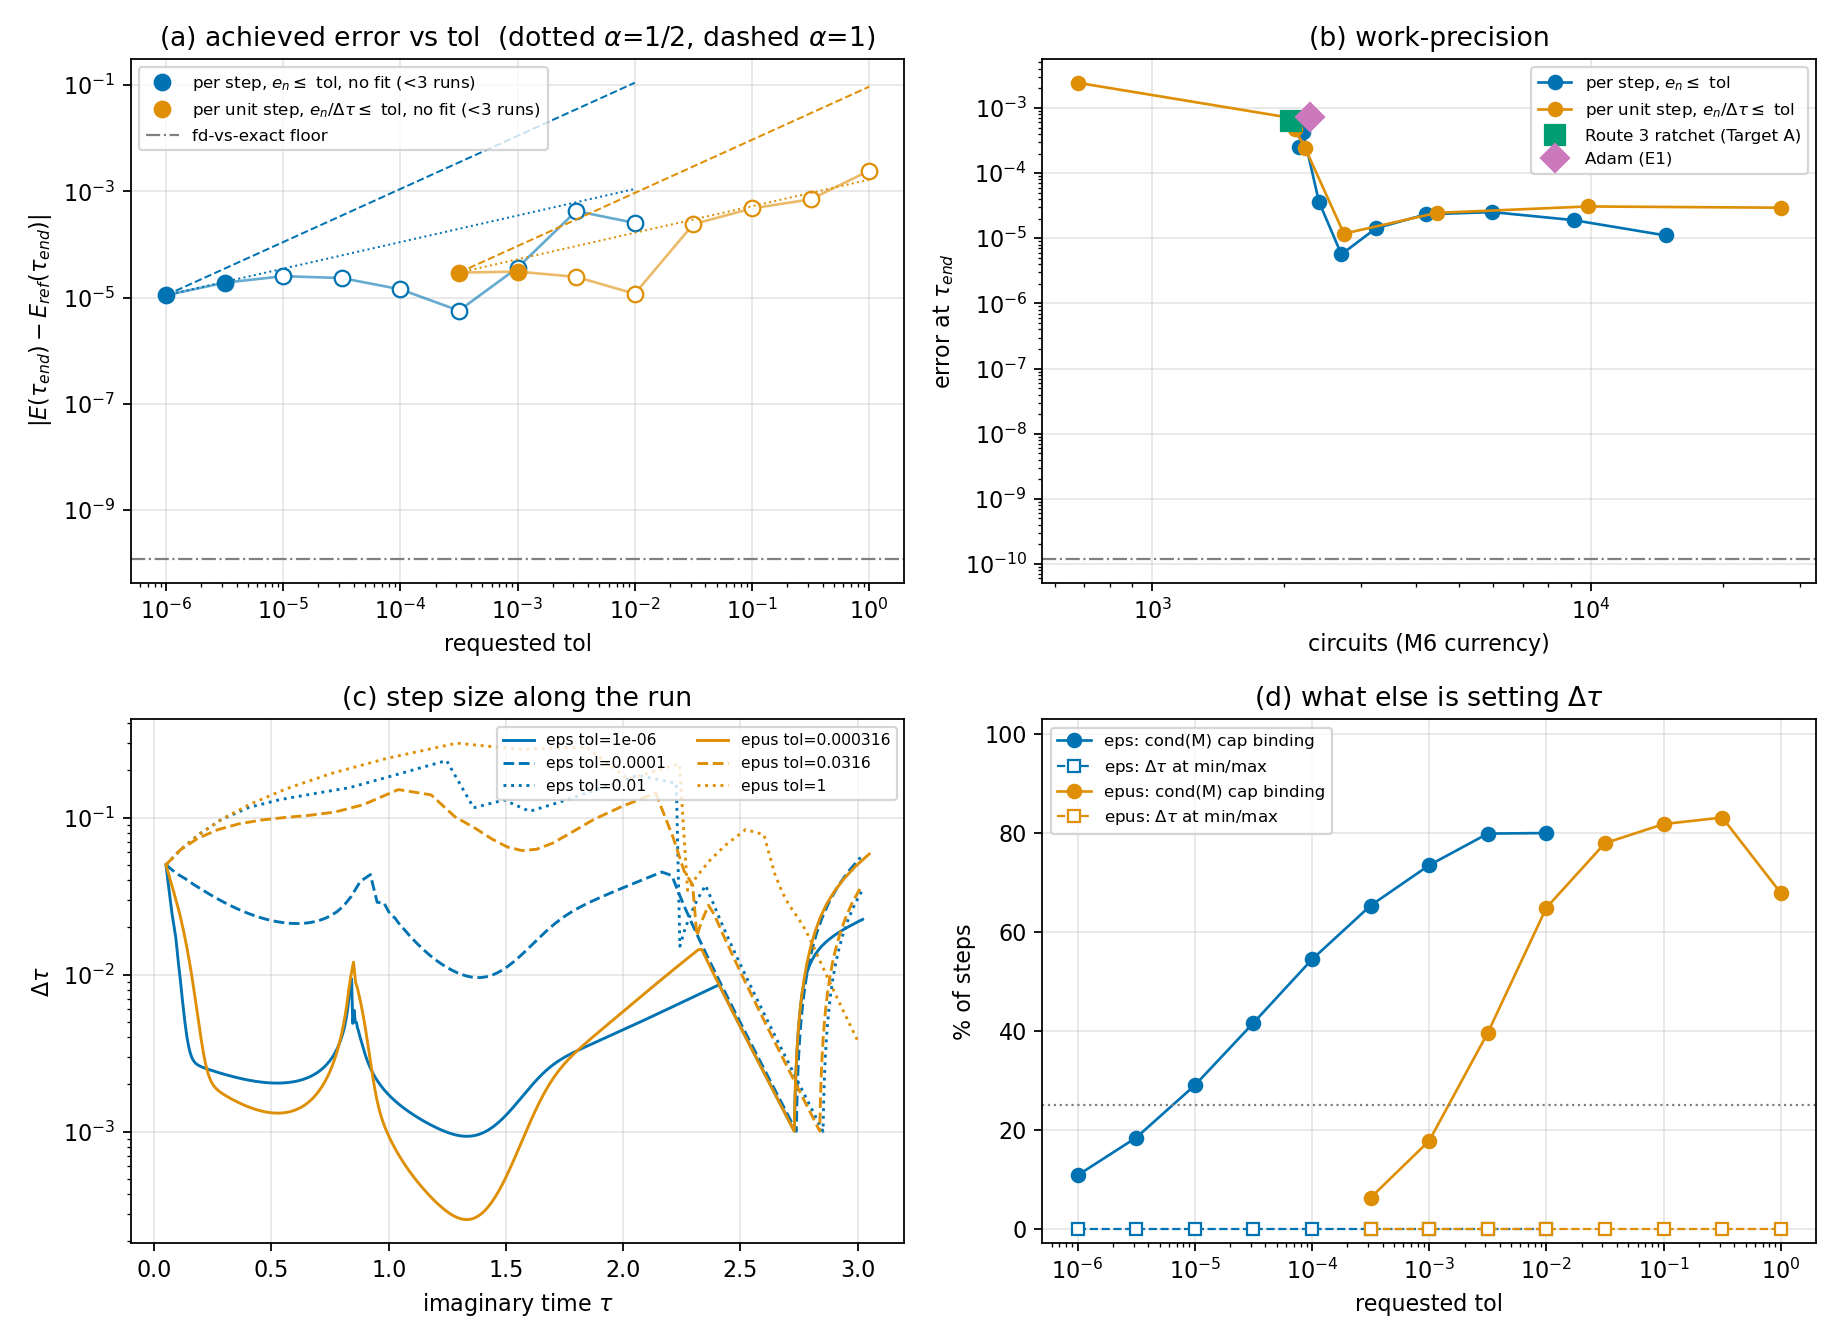
\includegraphics[width=0.78\textwidth]{p2_tol_proportionality}
\caption{P2 as registered. (a) End-point error against requested tolerance. Filled markers
are runs that qualify for the fit; the dotted and dashed lines are the $\alpha=1/2$ and
$\alpha=1$ predictions. (b) Work--precision in circuits, with the Route~3 and Adam anchors.
(c) Step size along selected runs. (d) Fraction of steps on which the $\cond(M)$ cap binds or
$\dt$ sits at a bound. The dotted line is the 25\% qualification limit.}
\label{fig:p2}
\end{figure*}

\begin{figure*}[t]
\centering
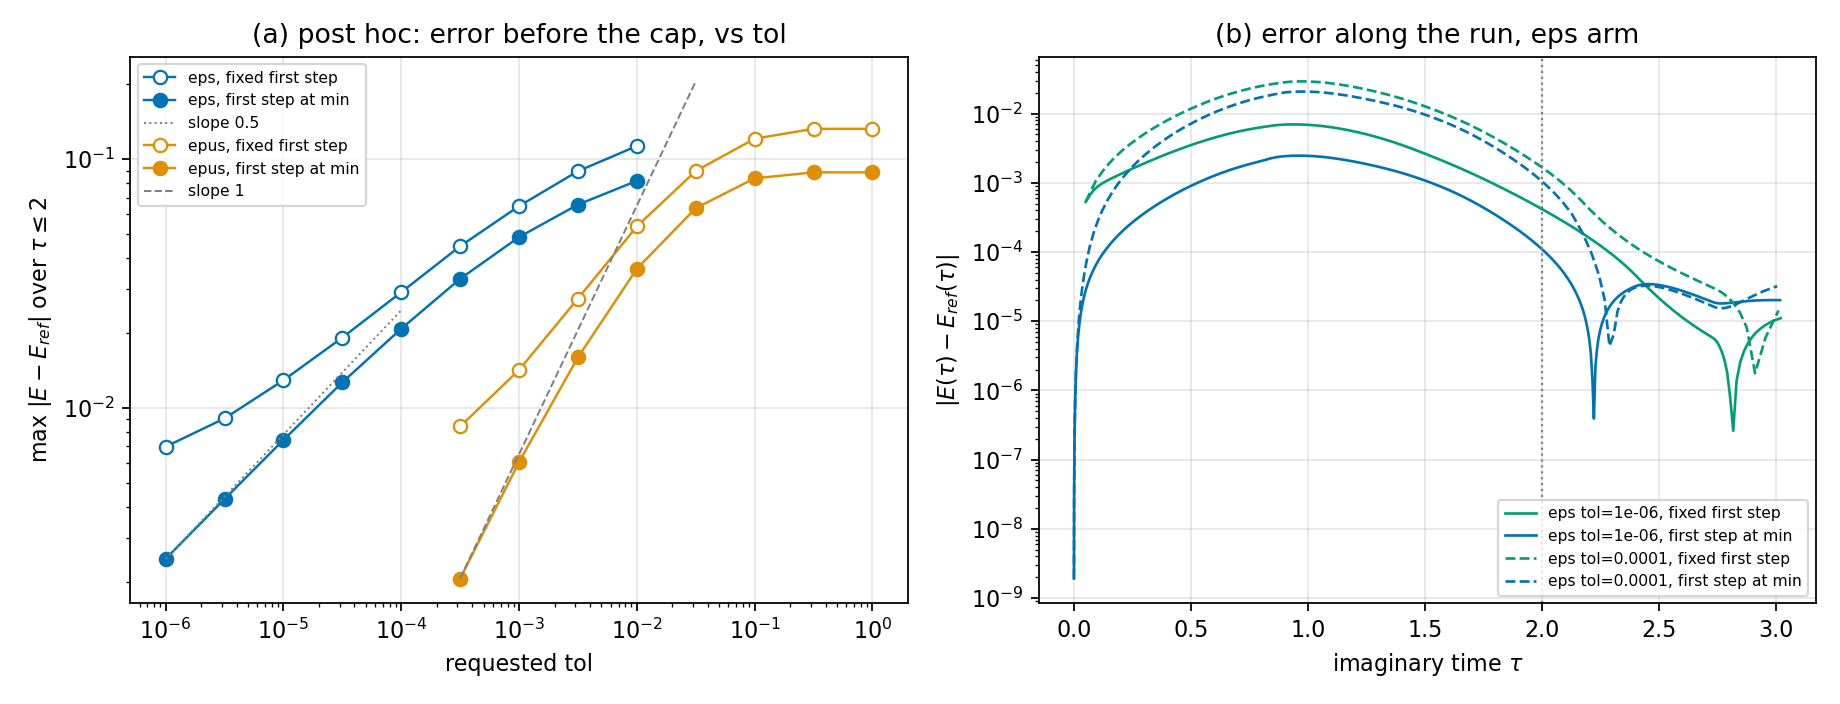
\includegraphics[width=0.78\textwidth]{p2_first_step_ablation}
\caption{P2 first-step ablation (post hoc). (a) Maximum error over $\tau\le2$, before the cap
engages, against $\tol$, with the fixed first step (open) and with the first step at the
minimum (filled). (b) Error along two EPS runs. The error peaks near $\tau\approx1$ and is then
damped by the flow.}
\label{fig:p2abl}
\end{figure*}

%% ===========================================================================
\section{Synthesis}
\label{sec:synthesis}

\subsection{Status of the claims}

Table~\ref{tab:claims} lists every substantive claim the project has made, with its present
status and where the evidence sits.

\begin{table*}[t]
\caption{Status of the project's claims at the close of Phase~V.}
\label{tab:claims}
\begin{ruledtabular}
\begin{tabular}{p{9.2cm}p{2.6cm}p{3.6cm}}
Claim & Status & Evidence \\
\midrule
Theorem~1 and the noisy-flow scaling of Ref.~\cite{QDP2024} hold & established & Sec.~\ref{sec:phase1}, T1/T4 \\
Theorem~2 overstates the hardware velocity error by exactly $2\times$ & established & Eq.~\eqref{eq:factor2}, Fig.~\ref{fig:t4} \\
QDP condition numbers (66.72; 20.22) & not reproduced & Sec.~\ref{sec:phase1}, T3 \\
9-parameter metric is structurally rank 6 of 9 & established & T3, P1 \\
Route~3 is $2.2\times$ closer to the floor than fixed Euler at 732 circuits & established & Target A \\
Debiasing with the corrected factor is exact per step & established & Target B \\
Debiasing improves full trajectories & not supported & Target B, Target D \\
Per-step debiasing error of 5--67\% (``surprise'') & retracted & F1/M1 \\
Noise floor near $p\approx10^{-3}$ & retracted & F4, Target D \\
Tight \rcond{} beats loose despite higher $\cond(M)$ & established & Target C, P1 \\
Adam-style memory improves the step law & not supported & G2, Table~\ref{tab:g2} \\
Adam is robust to noise (E2) & withdrawn & G3 \\
Adam improves stiffness handling (E3) & re-attributed to the cap & G6 \\
$s_e\le1$ & false & G2 \\
Energy-gate discrepancy is a zero-cost LTE estimator (ratio 2) & established & G5 \\
Estimator blind spot follows $\Delta\cond(M)$ & prediction failed & G5 \\
Route-3 stiffness is a chart singularity, not leakage or noise & established & P1 \\
PI law with explicit $\tol$ controls $e_n$ & established & P2 \\
End-point error scales as $\tol^{\alpha}$ & not fittable & P2 \\
Fixed first step and contraction explain the failure & post hoc & P2 ablation \\
Figures of Ref.~\cite{BeyondTrot2026} reproduce; four internal inconsistencies found & established & Table~\ref{tab:bt} \\
\end{tabular}
\end{ruledtabular}
\end{table*}

\subsection{Four ways the metric degenerates}

The project observed four distinct forms of degeneracy of the McLachlan metric. They
call for different treatment, and a single number such as $\cond(M)$ does not tell them apart.
\begin{enumerate}
\setlength\itemsep{0pt}
\item \textbf{Structural rank deficiency.} The ansatz has more parameters than the manifold has
  dimensions. The 9-parameter ansatz has exactly three gauge modes at roundoff throughout
  (T3, P1). They are harmless if the cutoff removes them, and they make any unregularized
  $\cond(M)$ meaningless.
\item \textbf{Boundary layer.} Repeated generators coincide at a special point, $t=0$ in
  Ref.~\cite{BeyondTrot2026}, with $\cond(g)\propto c_1^{-2}$. The layer is confined, and the
  result does not depend on how it is regularized (T6).
\item \textbf{Chart singularity (fold).} The map $\theta\mapsto\rho$ folds along the
  trajectory. One soft mode reaches $\sigma\sim10^{-7}$, the parameter speed diverges and the
  state speed stays bounded (P1). This is the stiffness the Route-3 cap handles.
\item \textbf{Zero-variance generator.} A gate whose generator has vanishing variance in the
  current state, here a CRZ with an almost deterministic control, drops out of $M$ (P1,
  Target~A control).
\end{enumerate}

\subsection{How the problems were found and handled}

The project's corrections share a pattern. Every retraction in Table~\ref{tab:claims} came from
a number that had been produced once and never re-derived by code: the debias factor, the
per-step ``surprise'', the noise-floor reading and the $s_e$ bound. Each was caught by an
audit that re-ran the claim against live code. The response has been procedural. Each claim
has one function, every quoted value is pinned with no adjustable tolerance, and from
Phase~V on predictions are registered before the run. Failed predictions are reported as
failures (P1: two of five; P2: five of six, for lack of a fit). Post-hoc analyses are labelled
as such.

%% ===========================================================================
\section{Scope of the evidence}
\label{sec:scope}

The results above hold under the following conditions, which are stated so that a reader can
calibrate them.
\begin{itemize}
\setlength\itemsep{0pt}
\item \textbf{One system.} All controller results are for H$_2$/STO-3G on two qubits with the
  two QDP ansätze. The Phase~IV results are for the models of Ref.~\cite{BeyondTrot2026}.
\item \textbf{No shot noise.} All expectation values are exact. The depolarizing model is
  deterministic, which is why E2 was withdrawn.
\item \textbf{Finite-difference derivatives} ($h=10^{-6}$), validated to about $10^{-10}$ and,
  in P1, against the exact state form. The finite-difference error reaches $1.1\times10^{-4}$ in
  energy after the fold.
\item \textbf{Chosen constants.} Every threshold in Table~\ref{tab:constants} was chosen for this work,
  and the conclusions are specific to them.
\item \textbf{Few seeds.} G2 uses two seeds, and E3 is a single run.
\item \textbf{Unresolved discrepancies.} The QDP condition numbers (T3) and the Fig.~3(b)
  reading (T5) have no identified cause on the paper's side. An error on the replication side is
  excluded as far as the 60-row convention scan allows.
\item \textbf{Unpinned checks.} The reparametrization test of Target~B and a few side checks in
  Phase~IV were run once and are labelled as such in the source notes.
\end{itemize}

%% ===========================================================================
\appendix

\section{Reproducibility}
\label{app:repro}

All code runs on Python~3.11 with PennyLane~0.45.1, NumPy and SciPy, in the project's
\texttt{qml-julia} environment. Paths are relative to the project folder.

\begin{table*}[t]
\caption{Scripts and pinned values.}
\label{tab:scripts}
\begin{ruledtabular}
\begin{tabular}{lp{10.2cm}p{4.6cm}}
Phase & Script & Pinned / check \\
\midrule
I   & \texttt{Replications/practical-limitations-qdp/replicate.py} & one function per target \\
II  & \texttt{Adam\_QITE/adam\_qite.py}, \texttt{verify\_audit.py} & 147 values, 0 drift, ${\approx}28$\,s \\
III & \texttt{Attack\_Route\_03/adaptive\_qite.py} (M1--M6) & \texttt{check\_eq\_b9\_self}, per-target seeds \\
IV  & \texttt{Replications/Beyond\_Trot/replicate.py --check} & 2 runs byte-identical \\
V   & \texttt{Route\_03\_and\_Beyond\_Trot/Proposal\_1/p1\_singularity.py} & 51 values, 0 drift \\
V   & \texttt{Route\_03\_and\_Beyond\_Trot/Proposal\_2/p2\_tol\_proportionality.py} & 93 values, 0 drift, byte-identical reruns \\
\end{tabular}
\end{ruledtabular}
\end{table*}

A \texttt{--check} run recomputes every pinned value and fails on any change. There is no
tolerance argument, so a deliberate perturbation of a pinned value makes the check fail.

\section{Derivations}
\label{app:derivations}

\subsection{The factor of two}
\label{app:factor2}

Let $\rho'=q\rho+(1-q)\mathbb 1/d$ denote both the differentiated state and the state inside
$\{H,\rho\}$. Then $\partial_k\rho'=q\,\partial_k\rho$ and $M'=q^2M$. For $Y$,
\[
\{H,\rho'\}-2\langle H\rangle'\rho' = q\{H,\rho\}+\tfrac{2(1-q)}{d}H-2\langle H\rangle'\rho' .
\]
Contracting with $\partial_k\rho'=q\,\partial_k\rho$ removes the last term because
$\Tr[\partial_k\rho\,\rho']=q\,\Tr[\partial_k\rho\,\rho]+\tfrac{1-q}{d}\Tr\,\partial_k\rho=0$ (for a
pure state $\Tr[\partial_k\rho\,\rho]=\tfrac12\partial_k\Tr\rho^2=0$). Since
$\Tr[\partial_k\rho\{H,\rho\}]=\partial_kE=-Y_k$ and $\Tr[\partial_k\rho\,H]=\partial_kE$,
\[
Y'_k=q^2Y_k+\tfrac{2q(1-q)}{d}Y_k .
\]
Hence $\thetadot'=M'^{+}Y'=\thetadot\,[1+2(1-q)/(dq)]$. For $d=4$ this is
$\thetadot[1+(1-q)/(2q)]$. If only $\partial_k\rho$ is noisy, as in Ref.~\cite{QDP2024},
$Y'=qY$ and $\thetadot'=\thetadot/q=\thetadot[1+(1-q)/q]$, which is Theorem~2.

\subsection{The update law cannot shrink the step}
\label{app:shrink}

The gate rejects exactly when $\hat e>1$ (Eq.~\eqref{eq:ehat}), and the controller is updated
only on accepted trials. Every observed $\hat e$ is therefore at most 1, and so are the EMAs
$\hat m_e$. With $s_e,k_I\ge0$, $\max(\hat m_e,\varepsilon)^{-s_ek_I}\ge1$. The growth factor
is at least 1 on every step, independently of the band.

\subsection{Ratio two against step doubling}
\label{app:ratio2}

Let one Euler step of size $\dt$ have local error $C\dt^2$. Two steps of $\dt/2$ have
$2C(\dt/2)^2=C\dt^2/2$, so the difference between the two, which is what step doubling
reports, is $C\dt^2/2$. The gate's $\Delta E_a-\Delta E_p$ is the full second-order remainder
of the energy along the Euler step, $C\dt^2$ read in energy. The ratio is therefore 2. The
remainder contains $\tfrac12\dt^2\,\thetadot^\top\nabla^2E\,\thetadot$ but not the part of
$\ddot\theta$ that comes from $\partial_\theta M^{+}$, which is the origin of the blind spot
in Sec.~\ref{sec:g5}.

\subsection{Tolerance exponents for EPS and EPUS}
\label{app:eps}

For a method of order $p$, the local error is $e_n\approx C\dt^{p+1}$. Under EPS the controller
holds $e_n\approx\tol$, so $\dt\propto\tol^{1/(p+1)}$. The global error, which is about
$T\,C\dt^{p}$, then scales as $\tol^{p/(p+1)}$, and the step count as $\tol^{-1/(p+1)}$. Under
EPUS it holds $e_n/\dt\approx\tol$, so $\dt^p\propto\tol$ and the global error scales as
$\tol^1$, with step count $\propto\tol^{-1/p}$. For explicit Euler ($p=1$) the predictions are
$\tol^{1/2}$ with circuit slope $-1/2$ (EPS) and $\tol^{1}$ with circuit slope $-1$ (EPUS). These
are the ``theory'' values in Table~\ref{tab:ablation}.

\section{Anticipated questions}
\label{app:qa}

\paragraph*{Why finite differences and not parameter-shift rules?} The derivative $\partial_k\rho$
of a density matrix is needed for $M$ and $Y$, and finite differences give it for any gate,
including under noise. The results were validated against the closed-form diagonal to
$8.9\times10^{-11}$ and, in P1, against the exact state form. The only place the difference
matters is after the fold, where it reaches $1.1\times10^{-4}$ in energy along the run; the
final error changes from $8.868181\times10^{-4}$ to $8.854194\times10^{-4}$.

\paragraph*{Why quote $\cond_F$ at all, if it depends on the cutoff?} Because the controller acts
on the regularized system that it actually solves. P1 shows that, at the tight cutoff, the
logged value equals the rank-6 condition number to $10^{-15}$, so it reads the physical soft
mode. The report always gives the cutoff with the number.

\paragraph*{Is the stiffness physical or an artifact of the ansatz?} It is a property of the
parametrization, a fold of $\theta\mapsto\rho$, and not of the state trajectory, whose speed
stays bounded (Table~\ref{tab:p1speed}). For an explicit integrator in $\theta$ it is real
stiffness all the same, and it caps the stable step.

\paragraph*{Could the replication gaps be implementation bugs?} The same code reproduces
the closed-form targets of both papers to $10^{-10}$--$10^{-16}$. Each gap is one-sided or
structural (T2, T3), survives a scan over conventions (60 rows for T3), or is resolved by a
single identifiable change on the paper's side (the $A\leftrightarrow B$ swap, the Eq.~(27)
normalization).

\paragraph*{Why does Adam act only on $\dt$?} Rescaling parameters individually changes the
direction of the update, so the integrator would no longer follow McLachlan's flow. The
controller was restricted to the one quantity a step controller is allowed to change.

\paragraph*{Why no shot noise?} The questions studied here (conditioning, step law, bias
factor) are deterministic, and adding shot noise would hide them. As a consequence, no claim
about robustness to stochastic noise is made (G3).

\paragraph*{Why does the end-point error fail as an accuracy measure?} Imaginary-time flow is
contractive. Errors made early are damped by two to three decades before the end
(Sec.~\ref{sec:phase5}), so the final error measures the damped remnant of early errors and
not the local accuracy the controller maintains.

\paragraph*{Why is Route~3 still the baseline, if it has no tolerance?} It wins every matched-budget comparison against Adam (Table~\ref{tab:g2}), and its
constants are fixed and documented. Several PI runs of P2 end closer to the reference than Route~3 at similar cost (Table~\ref{tab:p2}; e.g.\ $4.7659\times10^{-4}$ at 2115 circuits against $6.3181\times10^{-4}$ at 2069), but on one seed and with an end-point error that is not monotone in the tolerance, so no advantage is claimed. A second seed at matched circuits (P2b) is the test.

%% ===========================================================================
\begin{thebibliography}{9}

\bibitem{QDP2024}
G.~Saxena, A.~Shalabi, and T.~H.~Kyaw,
Practical limitations of quantum data propagation on noisy quantum processors,
\href{https://doi.org/10.1103/PhysRevApplied.21.054014}{Phys. Rev. Applied \textbf{21}, 054014 (2024)},
\href{https://arxiv.org/abs/2306.13046}{arXiv:2306.13046}.

\bibitem{BeyondTrot2026}
I.~Assi, M.~Vogl, M.~Kumari, and J.~P.~F.~LeBlanc,
Beyond Trotterization: Variational product formulas for quantum simulation,
\href{https://doi.org/10.1103/941r-ql3g}{Phys. Rev. B \textbf{113}, 214314 (2026)},
\href{https://arxiv.org/abs/2511.15124}{arXiv:2511.15124}.

\bibitem{Angles2025}
A.~Anglés-Castillo, L.~Ion, T.~Pandit, R.~Gomez-Lurbe, R.~Martínez, and M.~A.~Garcia-March,
Understanding quantum imaginary time evolution and its variational form,
\href{https://arxiv.org/abs/2510.02015}{arXiv:2510.02015} (2025).

\bibitem{Arulandu2026}
A.~Arulandu, J.~M.~Martyn, and I.~L.~Chuang,
Trading imaginary time for randomness in ground state preparation,
\href{https://arxiv.org/abs/2608.00443}{arXiv:2608.00443} (2026).

\bibitem{Motta2020}
M.~Motta, C.~Sun, A.~T.~K.~Tan, M.~J.~O'Rourke, E.~Ye, A.~J.~Minnich, F.~G.~S.~L.~Brandão, and
G.~K.-L.~Chan,
Determining eigenstates and thermal states on a quantum computer using quantum imaginary time
evolution, Nat. Phys. \textbf{16}, 205 (2020).

\bibitem{McArdle2019}
S.~McArdle, T.~Jones, S.~Endo, Y.~Li, S.~C.~Benjamin, and X.~Yuan,
Variational ansatz-based quantum simulation of imaginary time evolution,
npj Quantum Inf. \textbf{5}, 75 (2019).

\bibitem{Memo}
Adaptive time-stepping for variational QITE: An RKF-type controller with a hardware-noise floor,
internal memo, LG Electronics Toronto AI team (unpublished).

\end{thebibliography}

\end{document}
